%\documentclass[xcolor=table,handout,compress]{beamer}
\documentclass[xcolor=table]{beamer}
%--------------------------------------------------------------------------
% Common packages
%--------------------------------------------------------------------------
\usepackage[english]{babel}
\usepackage{pgfpages} % required for notes on second screen
\usepackage{graphicx}
\usepackage{subfigure}
\usepackage{multicol}
\usepackage[normalem]{ulem}

\usepackage{tabularx,ragged2e}
\usepackage{booktabs}
\usepackage{marvosym}

\makeatletter
\let\beamer@writeslidentry@miniframeson=\beamer@writeslidentry
\def\beamer@writeslidentry@miniframesoff{%
  \expandafter\beamer@ifempty\expandafter{\beamer@framestartpage}{}% does not happen normally
  {%else
    % removed \addtocontents commands
    \clearpage\beamer@notesactions%
  }
}
\newcommand*{\miniframeson}{\let\beamer@writeslidentry=\beamer@writeslidentry@miniframeson}
\newcommand*{\miniframesoff}{\let\beamer@writeslidentry=\beamer@writeslidentry@miniframesoff}
\makeatother


%--------------------------------------------------------------------------
% Load theme
%--------------------------------------------------------------------------
\usetheme{hri}

\usepackage{tikz}
\usetikzlibrary{patterns,shapes,fpu,fit,calc,mindmap,backgrounds,positioning,svg.path}

\tikzset{
  invisible/.style={opacity=0},
  visible on/.style={alt={#1{}{invisible}}},
  alt/.code args={<#1>#2#3}{%
    \alt<#1>{\pgfkeysalso{#2}}{\pgfkeysalso{#3}} % \pgfkeysalso doesn't change the path
  },
}

%% Neat trick to have only one navigation bullet per subsection
%% http://tex.stackexchange.com/questions/64333/one-navigation-bullet-per-subsection-with-subsection-false-in-custom-beamer-them
%\usepackage{etoolbox}
%\makeatletter
%\patchcmd{\slideentry}{\advance\beamer@xpos by1\relax}{}{}{}
%\def\beamer@subsectionentry#1#2#3#4#5{\advance\beamer@xpos by1\relax}%
%\makeatother
%%%%%%%%%%%%%%%%%%%%%%%%%%%%%%%%%%%%%%%

\graphicspath{{figs/}}

% for model of anthopomorphism
\newcommand{\IPA}{{$\mathcal{A}_0$~}}
\newcommand{\SLA}{{$\mathcal{A}_\infty$~}}
\newcommand{\sla}{{\mathcal{A}_\infty}}
\newcommand{\AntMax}{{$\mathcal{A}_{max}$~}}
\newcommand{\antMax}{{\mathcal{A}_{max}}}

% for HATP plans
\newcommand{\hatpaction}[3]{#1\\\textsf{\scriptsize #2,}\\\textsf{\scriptsize #3}}
\newcommand{\stmt}[1]{{\footnotesize \tt  #1}}

% for mutual modelling
\newcommand{\Mmodel}[3]{{\mathcal{M}(#1, #2, #3)}}
\newcommand{\model}[3]{{$\mathcal{M}(#1, #2, #3)$}}
\newcommand{\Model}[3]{{$\mathcal{M}^{\circ}(#1, #2, #3)$}}

% typeset logical concept
\newcommand{\concept}[1]{{\scriptsize \texttt{#1}}}

\newcommand{\backbutton}{\hfill\hyperlink{appendix}{\beamerreturnbutton{Supplementary material}}}
%--------------------------------------------------------------------------
% General presentation settings
%--------------------------------------------------------------------------
\title{\Large Socially-driven Autonomous Robots\newline for Real-World Human-Robot Interactions}
\subtitle{~}
\date{{\bf KTH seminar} | 06 Apr 2021}
\author{Séverin Lemaignan}
\institute{{\bf Bristol Robotics Lab}\\University of the West of England}

%--------------------------------------------------------------------------
% Notes settings
%--------------------------------------------------------------------------
%\setbeameroption{show notes on second screen}
%\setbeameroption{hide notes}

\begin{document}


%%%%%%%%%%%%%%%%%%%%%%%%%%%%%%%%%%%%%%%%%%%%%%%%%%%%%%%%


%%%%%%%%%%%%%%%%%%%%%%%%%%%%%%%%%%%%%%%%%%%%%%%%%%%%%%%%

\licenseframe{github.com/severin-lemaignan/presentation-research}

\maketitle
%\imageframe{titlepage}

{\fullbackground{europe_map}
\begin{frame}{Short bio}

    \begin{columns}
        \begin{column}{0.7\linewidth}

    \begin{itemize}
        \item \textbf{2008--2012} Joint French (LAAS-CNRS) German (TU
            Munich) PhD\\
            \begin{itemize}
                \item AI \& Cognitive Robotics
            \end{itemize}

        \item \textbf{2013--2015} Post-doc at EPFL
            \begin{itemize}
                \item Child-robot interactions
            \end{itemize}

        \item \textbf{2015-2018} Post-doc + lecturer at Plymouth University, UK
            \begin{itemize}
                \item EU Marie Curie fellowship
                \item Social Cognition in Robotics
            \end{itemize}

        \item \textbf{2018--2021} Associate Prof. at Bristol Robotics Lab

        \item \textbf{2021--} ...??!

    \end{itemize}

    \end{column}
        \begin{column}{0.4\linewidth}
    \end{column}
    \end{columns}
            
\end{frame}
}

\imageframe{my_background/00}




\begin{frame}<1-7>[label=soro]{Social Robotics}
    \centering

    \begin{columns}
        \begin{column}{0.7\linewidth}

            \only<1>{
                Creating interactive robots that are \textbf{embedded and
                understand their (human) social context}; \textbf{generate and adopt appropriate
                social behaviours}; have a \textbf{positive impact on human
                society}.

                \vspace{2em}
                $\Rightarrow$ designing and implementing the \textbf{assistant and
                companion robots} for  tomorrow.

                \vspace{2em}
                $\Rightarrow$ direct impact on ageing society, education, customer service;
                \textbf{major socio-economic
                challenge}; \textbf{European priority}.
            }

            \only<2->{
                \textbf{Major scientific challenges}:

                \begin{itemize}
                    \item<2-> Model open-ended, underspecified situations; rich
                        semantics; complex social dynamics;
                    \item<3-> Close the interaction loop;
                    \item<4-> Understand and sustain long-term autonomous social interactions;
                    \item<5-> Real-world algorithmic robustness;
                    \item<6-> Complex ethical landscape;
                    \item<7-> $\Rightarrow$ cross-disciplinary \& holistic approach required
                \end{itemize}


                \uncover<8>{
                \vspace{1em}


                \setbeamercolor{hriSec1Demo}{bg=hriSec3Dark,fg=white}
                \begin{beamercolorbox}[wd=\linewidth,ht=8ex,dp=0.7ex]{hriSec1Demo}
                    \large \bf \centering
                    Socially-Driven Autonomous Robots \\
                    for \\
                    Real-world Human-Robot Interactions
                \end{beamercolorbox}
            }


            }
        \end{column}
        \begin{column}{0.35\linewidth}
            \begin{center}
                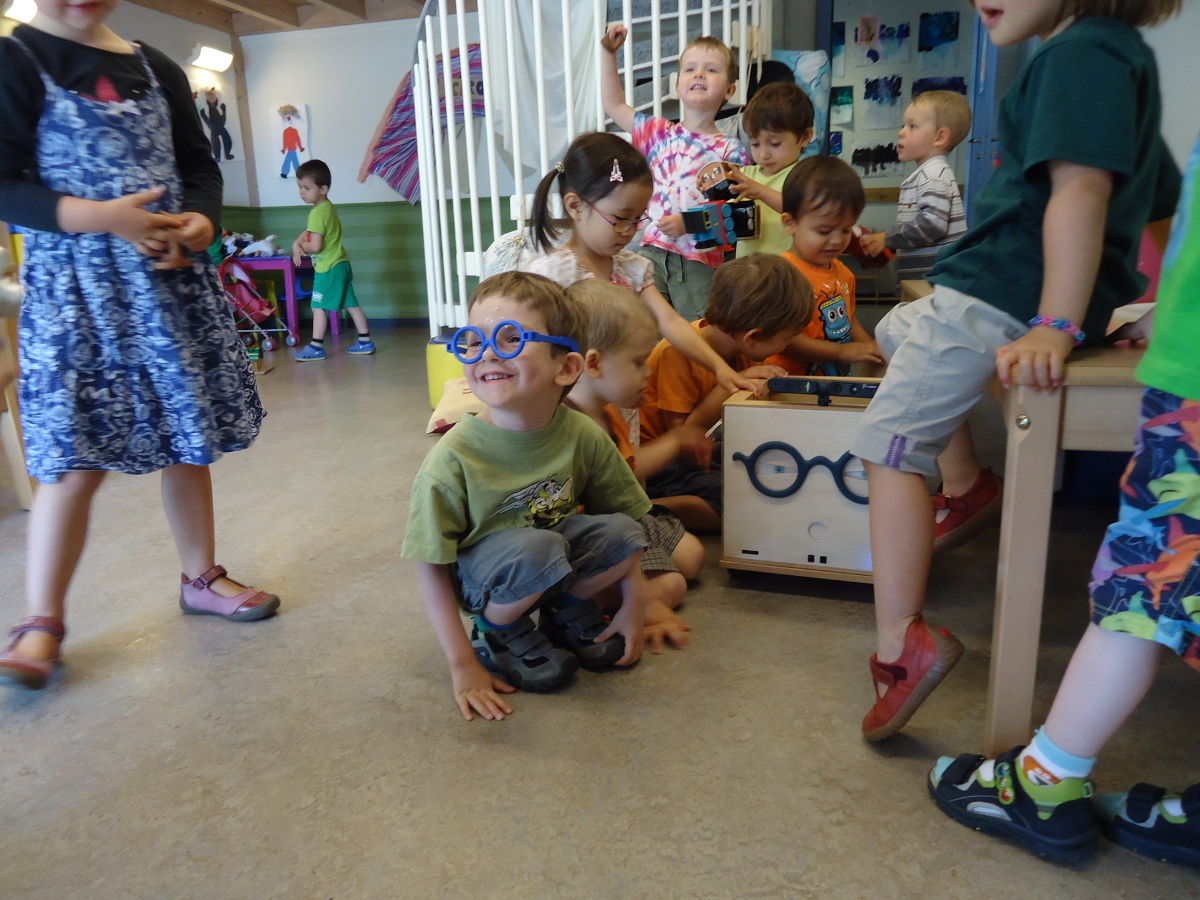
\includegraphics[trim=15cm 0 11cm 0,clip,width=\linewidth]{ranger/ranger_funny_glasses}
            \end{center}
        \end{column}
    \end{columns}

    %    \pause
    %    How to balance long-term \emph{social autonomy} (goal-driven architecture)
    %    with \emph{human oversight}?
\end{frame}

{
    \paper{Baxter, Lemaignan, Trafton {\bf Workshop on Cognitive Architectures for Social HRI} -- HRI 2016}
\begin{frame}<5>[label=mindmap]
\centering
        \resizebox{!}{0.8\paperheight}{%
            \begin{tikzpicture}[
                    >=latex,
                every edge/.style={<-, draw, very thick}]
        

            \path[small mindmap, 
                level 1 concept/.append style={sibling angle=360/6}, 
                level 2 concept/.append style={sibling angle=60}, 
                concept color=hriWarmGreyDark,text=white]
            node[concept color=white, text=hriWarmGreyDark, visible on=<1-5>] {\bf Social\\Cognition in HRI}
            [clockwise from=30]
            child[concept] { node[concept] (percept) {Perception of Human's State}
                [clockwise from=120]
                child[concept] { node[concept]
                (emotions) {Empathy Emotions} }
                child[concept] { node[concept] (attention) {Attention} }
                child[concept] { node[concept] (mmodel) {Inference of mental models} };
            }
            child[concept,grow=-45, visible on=<2->] { node[concept] (knowledge) {Social Knowledge} 
                [counterclockwise from=-140]
                child[concept] { node[concept] (soc-rules) {Social rules} }
                child[concept] { node[concept] (soc-ctxt) {Social context} }
                child[concept] { node[concept] (memory) {Social memory} }
                child[concept] { node[concept] (common-sense) {Common-sense} };
            }
            child[concept, grow=-120,visible on=<3->] { node[concept] (comm) {Communication} 
                [counterclockwise from=180]
                child[concept] { node[concept] (dialog) {Verbal} }
                child[concept] { node[concept] (non-verbal) {Non-verbal} };
            }
            child[concept,grow=180,visible on=<4->] { node[concept] (dynamics) {Interaction Dynamics} 
                [clockwise from=180]
                child[concept] { node[concept] (long-term) {Long-term interaction} };
            }
            child[concept, grow=120,visible on=<5->] { node[concept] (action) {Performing with humans} 
                [counterclockwise from=80]
                child[concept] { node[concept] {Action, behaviour recognition} }
                child[concept] { node[concept] {Intention reading} }
                child[concept] { node[concept] (joint-action) {Joint actions} };
            };


        \end{tikzpicture}
    }
\end{frame}
}

%
%\begin{frame}{What have we been up to over the last 3 years?}
%    \begin{center}
%        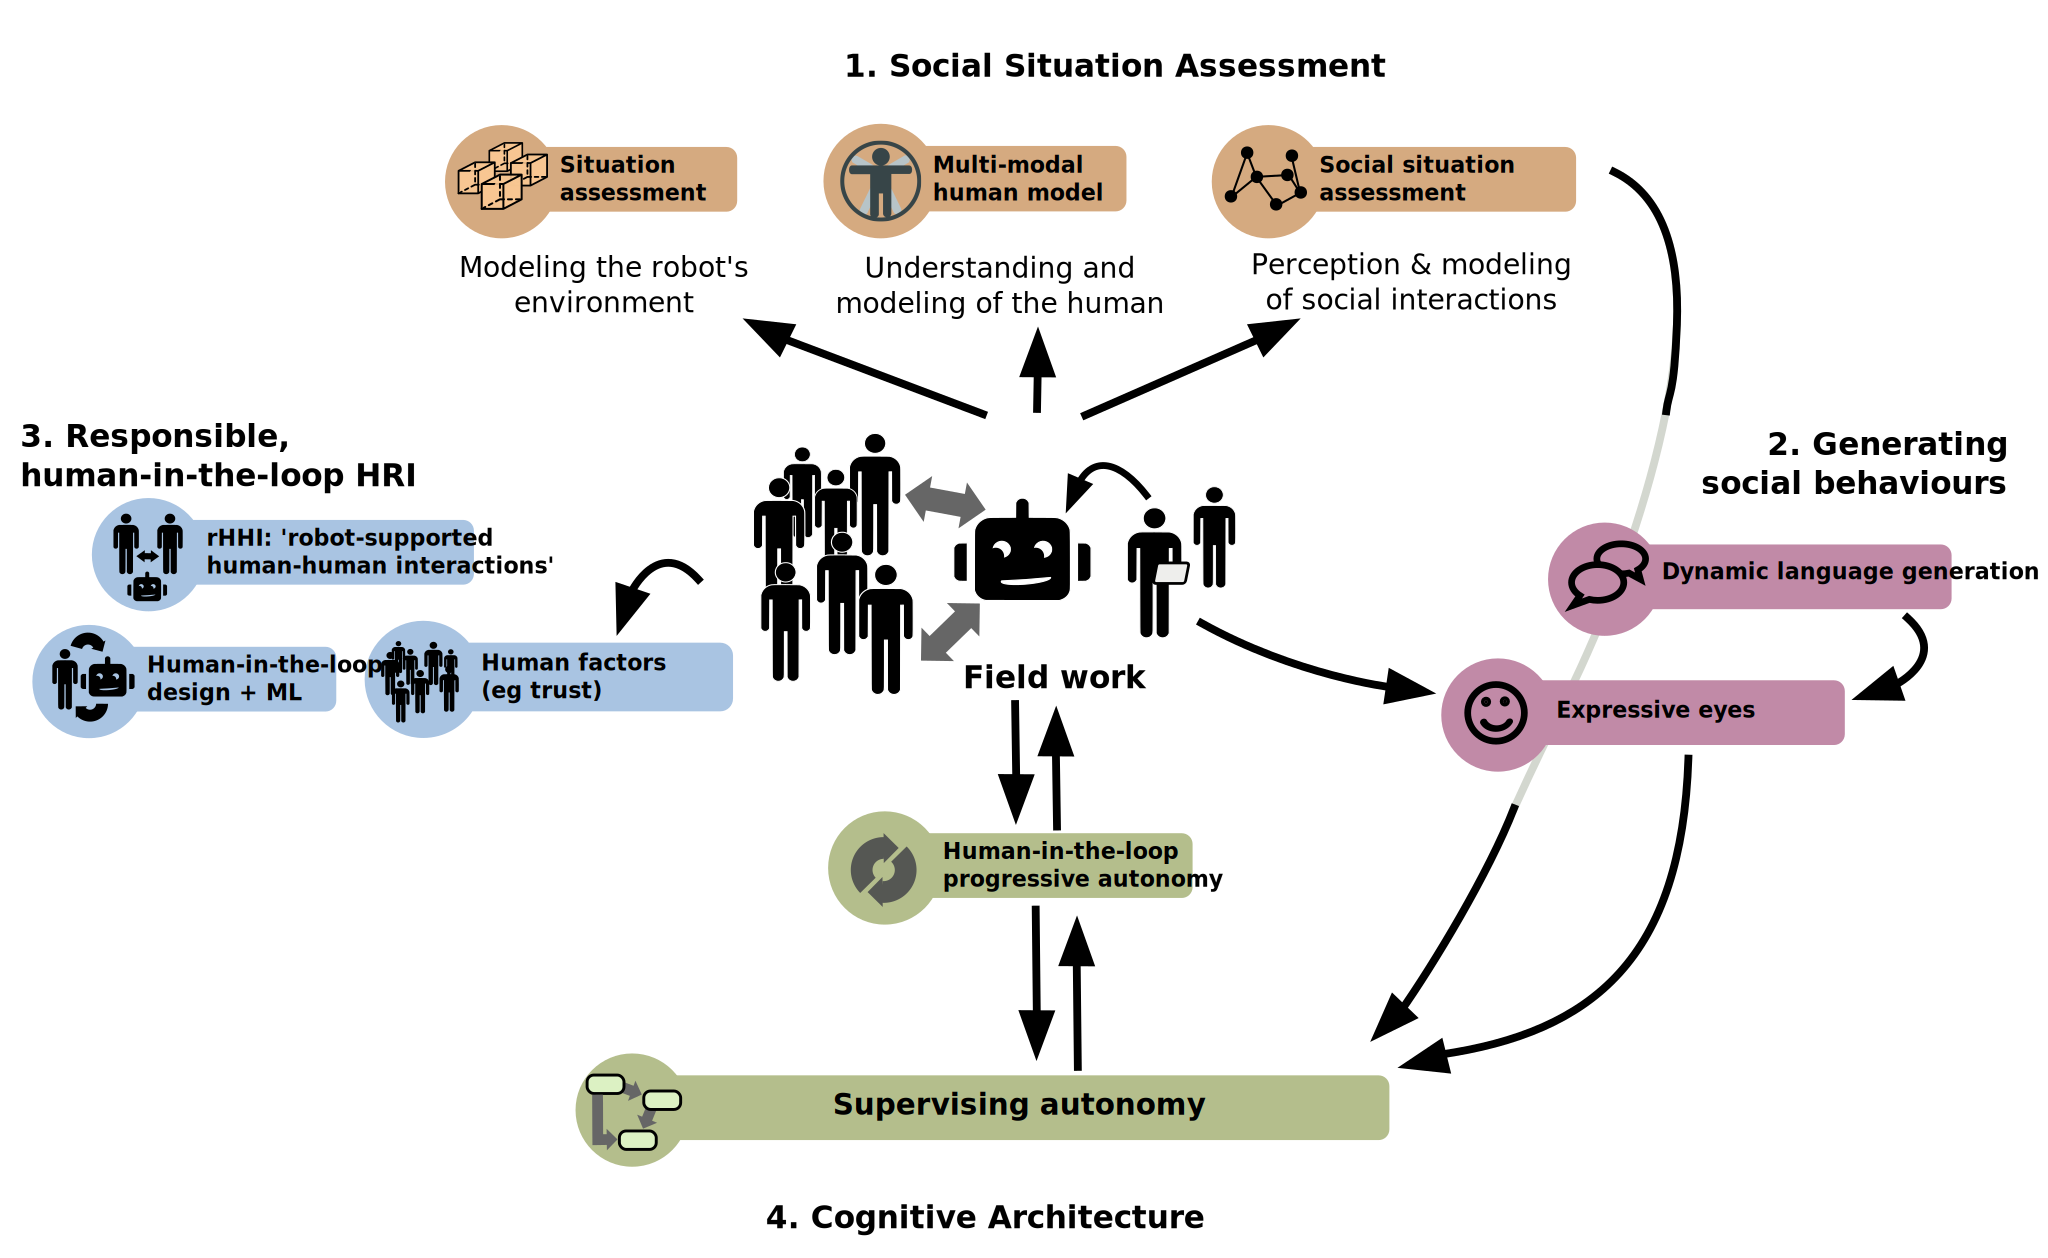
\includegraphics[width=\linewidth]{architectures/sota2021}
%    \end{center}
%\end{frame}

\imageframe[scale=0.9]{figs/echos-big-picture}
\miniframesoff
\imageframe[scale=0.9]{figs/big-picture-path1}
\imageframe[scale=0.9]{figs/big-picture-path2}
\imageframe[scale=0.9]{figs/big-picture-path3}
\imageframe[scale=0.9]{figs/big-picture-path4}
\imageframe[scale=0.9]{figs/big-picture-path5}
\imageframe[scale=0.9]{figs/big-picture-path6}
\imageframe[scale=0.9]{figs/big-picture-path7}
\imageframe[scale=0.9]{figs/big-picture-path8}
\imageframe[scale=0.9]{figs/big-picture-path9}
\miniframeson

\section[Social Situations]{from Social situation assessment...}


{
    \paper{Sallami et al. \textbf{Simulation-based physics reasoning for
    consistent scene estimation in an HRI context} IROS 2019]

    [Lemaignan et al. \textbf{Artificial Cognition for Social Human-Robot
    Interaction: An Implementation} Artificial Intelligence 2017
    }

    \begin{frame}{Situation assessment}

        \begin{columns}
            \begin{column}{0.5\linewidth}
                    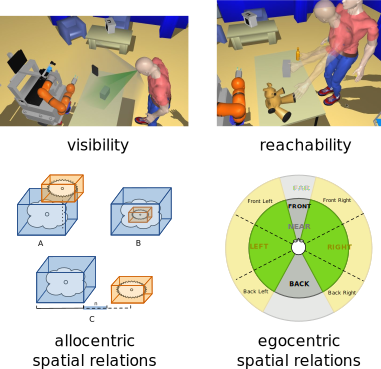
\includegraphics[width=0.8\linewidth]{figs/sit-ass/spark_vert}

            \end{column}
            \begin{column}{0.5\linewidth}
                \video[0.56]{\linewidth}{figs/sit-ass/underworlds.mp4?start=20&autostart}
            \end{column}
        \end{columns}


        \badge[caption=Yoan Sallami]{colleagues/yoan}
    \end{frame}
}

{
    \paper{Sallami et al. \textbf{The Unexpected Daily Situations Dataset: A New
Benchmark for Socially-Aware Assistive Robots} HRI LBR 2020}

\begin{frame}{Common-sense: unexpected situations}
    \begin{center}

        UDS: the Unexpected Daily Situations dataset


        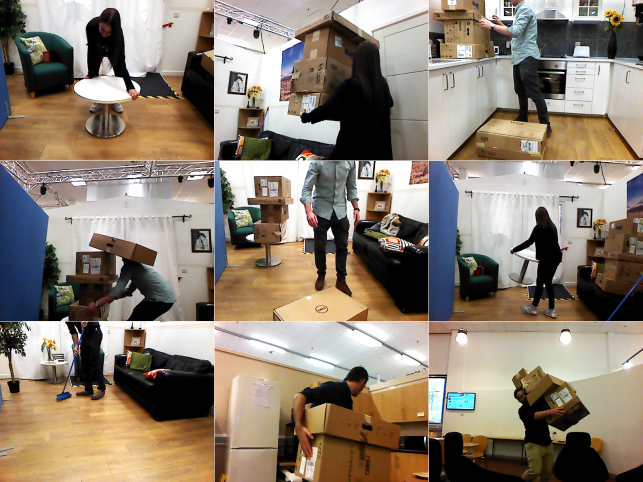
\includegraphics[width=0.7\linewidth]{uds/mosaic}

        {\scriptsize (idea borrowed from dev. psychologists Warneken and
        Tomasello)}

    \end{center}

    \badge[caption=Yoan Sallami]{colleagues/yoan}
\end{frame}
}

\videoframe[0.56]{figs/uds/uds.mp4?autostart}

{

    \paper{Mohamed, Lemaignan \textbf{ROS for Human-Robot Interaction} Arxiv
    2021 (under review IROS)}

\begin{frame}{ROS4HRI}
    \begin{center}
        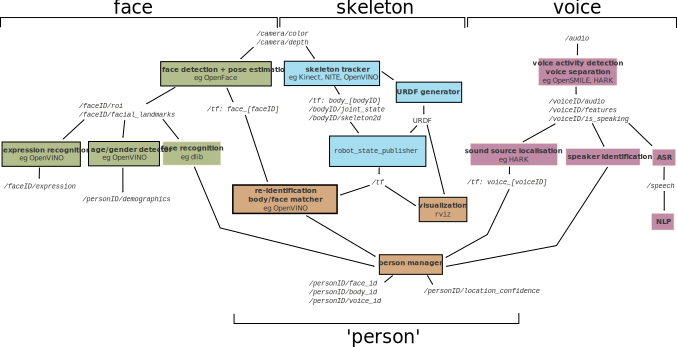
\includegraphics[width=\columnwidth]{architectures/ros4hri-pipeline}
    \end{center}
    ROS4HRI: first integrated, multi-modal, ROS-based pipeline for social signal
    processing in robotics

    \badge[caption=Youssef Mohamed]{colleagues/youssef}
\end{frame}
}


\section[Internal state]{...to internal state...}

{
    \paper{Webb, Mohamed, Lemaignan \textbf{Framing the Challenge of Social
    Interaction Modelling} HRI LBR 2021}

\begin{frame}{Social modeling}
    \begin{center}
        
\includegraphics[width=0.95\linewidth]{figs/social-interactions/social-complexity}
    \end{center}

    \onslide<2> {
        \begin{itemize}
            \item multi-modal
            \item dynamic
            \item only partially observable
            \item complex pipeline; hard to make it robust
        \end{itemize}
    }

    \badge[caption=Nicola Webb]{colleagues/nicola}
\end{frame}
}

%%%%%%%%%%%%%%%%%%%%%%%%%%%%%%%%%%%%%%%%%%%%%%%%%%%%%%%%%%%%%%%%%%%%%%%%%%%%%%%%%%%%%%%%%



%\imageframe[color=black]{social-interactions/social-interactions.pdf}

{
    \paper{Lemaignan et al. \textbf{The PInSoRo dataset: Supporting the
    data-driven study of child-child and child-robot [...]} PLOS One 2018}


\begin{frame}{Deciphering internal state}
    \begin{columns}
        \begin{column}{0.5\linewidth}
            \vspace{0.4cm}
            \video{\columnwidth}{figs/pinsoro/annotations.mp4?autostart}
        \end{column}
        \begin{column}{0.5\linewidth}
            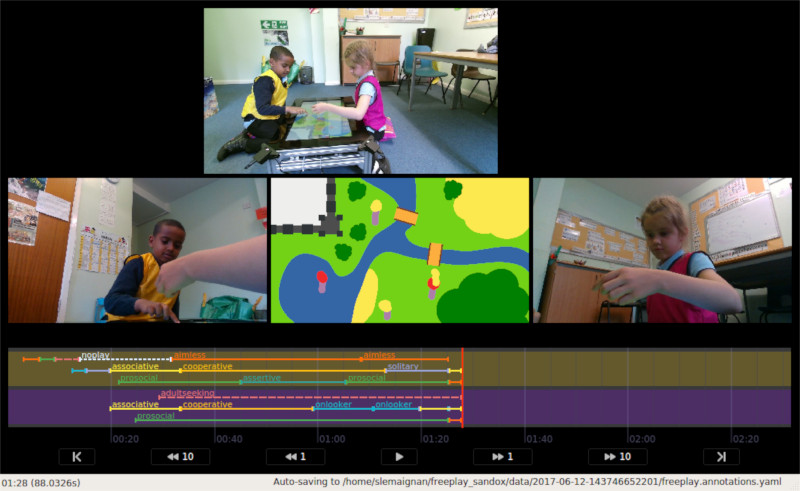
\includegraphics[width=\columnwidth]{pinsoro/annotator.jpg}
            %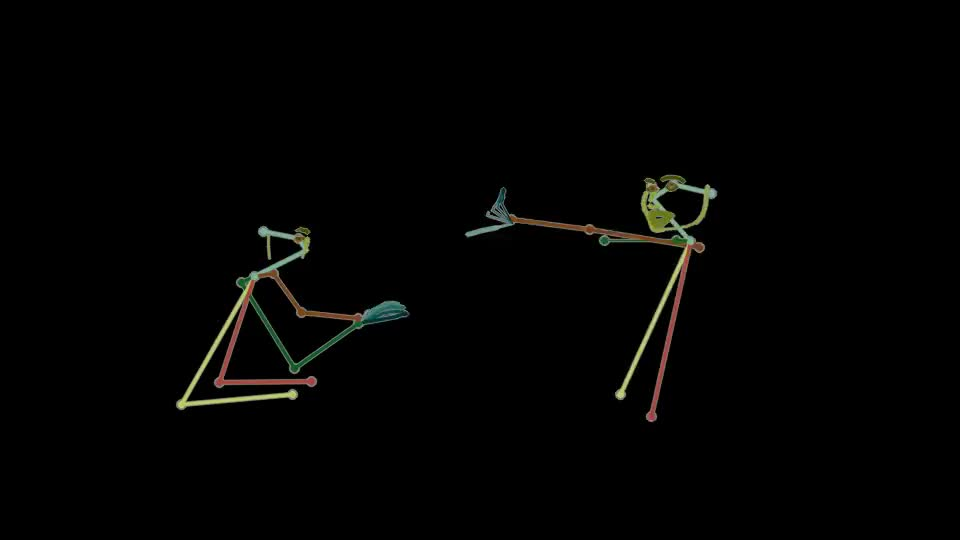
\includegraphics[width=\columnwidth]{kinematics_social_dynamics/clip_skel_05_thumb.jpg}

        \end{column}
    \end{columns}
%    \vspace{0.5cm}
\begin{columns}
    \begin{column}{0.5\linewidth}
        {\scriptsize
        \begin{itemize}
            \item PInSoRo dataset: 45h+ and 2M frames of annotated natural
                interactions. \url{freeplay-sandbox.github.io}
            \item first-in-kind dataset for data-driven study of social
                interactions in robotics
            \item new data analysis techniques to estimate internal state from body language
        \end{itemize}
        }
    \end{column}
    \begin{column}{0.5\linewidth}
            %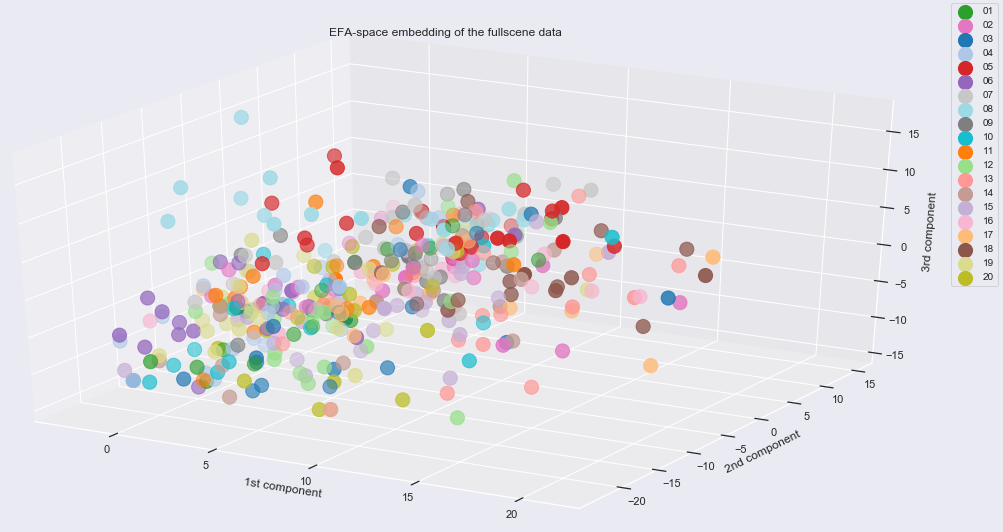
\includegraphics[trim=1cm 0 4cm 0,clip,width=\columnwidth]{kinematics_social_dynamics/efa-embeddings.png}
            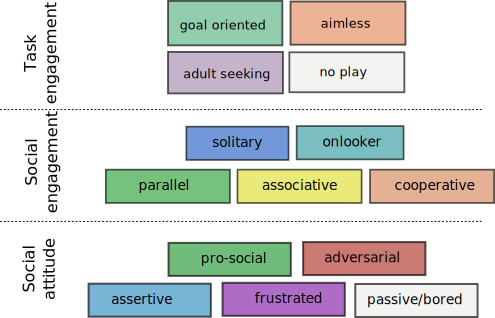
\includegraphics[width=\columnwidth]{pinsoro/coding-scheme}
    \end{column}
\end{columns}

    \badge[caption=Maddy Bartlett]{colleagues/maddy}
\end{frame}
}

\videoframe[0.56]{figs/kinematics_social_dynamics/clip_skel_01.mp4}

%%%%%%%%%%%%%%%%%%%%%%%%%%%%%%%%%%%%%%%%%%%%%%%%%%%%%%%%

\videoframe[0.56]{figs/kinematics_social_dynamics/clip_01.mp4}

%%%%%%%%%%%%%%%%%%%%%%%%%%%%%%%%%%%%%%%%%%%%%%%%%%%%%%%%

\videoframe[0.56]{figs/kinematics_social_dynamics/clip_skel_05.mp4}

%%%%%%%%%%%%%%%%%%%%%%%%%%%%%%%%%%%%%%%%%%%%%%%%%%%%%%%%

\videoframe[0.56]{figs/kinematics_social_dynamics/clip_05.mp4}

\imageframe[caption={200 participants, 4 clips each, on MTurk}]{kinematics_social_dynamics/questionnaire.png}
%\imageframe{kinematics_social_dynamics/dataset.png}
%\imageframe[caption={For each construct, calculate $\Delta$ and $\Sigma$}]{kinematics_social_dynamics/dataset-sumdiff.png}

{
    \paper{Bartlett et al. \textbf{What Can You See? Identifying Cues on
Internal States from the Kinematics [...]} FrontiersIn 2019}

\begin{frame}{EFA: Exploratory Factor Analysis}

\tiny
\rowcolors{2}{gray!25}{white}
\begin{tabular}{lrr|rr|rr}

    {} & \multicolumn{2}{l}{\bf Factor 1\onslide<2->{: imbalance}} &
    \multicolumn{2}{l}{\bf Factor 2\onslide<2->{: (negative) valence}} & \multicolumn{2}{l}{\bf
    Factor 3\onslide<2->{: engagement}} \\
    {} & \emph{full-scene} &  \onslide<3->{\emph{mov.-alone}} & \emph{full-scene} &
    \onslide<3->{\emph{mov.-alone}} & \emph{full-scene} &
    \onslide<3->{\emph{mov.-alone}} \\
\midrule
    \textbf{$\Delta$ Sad       } &      0.41 &  \only<3->{0.52} &           &                  &           &       \\
    \textbf{$\Sigma$ Sad       } &           &                  &      0.72 & \only<3->{ 0.53} &           & \only<3->{ 0.49} \\
    \textbf{$\Delta$ Happy     } &      0.49 &  \only<3->{0.53} &           &                  &           & \\
    \textbf{$\Sigma$ Happy      } &           &                 &           & \only<3->{-0.51} &     -0.55 & \\
    \textbf{$\Delta$ Angry     } &      0.40 &  \only<3->{0.62} &           &                  &           & \\
    \textbf{$\Sigma$ Angry      } &           &                 &      0.81 & \only<3->{ 0.85} &           & \\
    \textbf{$\Delta$ Excited   } &      0.53 &  \only<3->{0.63} &           &                  &           & \\
    \textbf{$\Sigma$ Excited    } &           &                 &           &                  &     -0.71 & \\
    \textbf{$\Delta$ Calm      } &      0.45 &  \only<3->{0.63} &           &                  &           & \\
    \textbf{$\Sigma$ Calm       } &           &  \only<3-> {  } &           & \only<3->{-0.45} &           & \\
    \textbf{$\Delta$ Friendly  } &      0.69 &  \only<3->{0.56} &           &                  &           & \\
    \textbf{$\Sigma$ Friendly   } &           &  \only<3->{   } &           & \only<3->{-0.60} &     -0.43 & \\
    \textbf{$\Delta$ Aggressive} &      0.78 &  \only<3->{0.79} &           &                  &           & \\
    \textbf{$\Sigma$ Aggressive } &           &  \only<3->{   } &      0.80 & \only<3->{ 0.72} &     -0.36 & \\
    \textbf{$\Delta$ Engaged   } &           &  \only<3->{0.39} &           &                  &      0.65 & \only<3->{ 0.52} \\
    \textbf{$\Sigma$ Engaged    } &           &  \only<3->{   } &           &                  &     -0.64 & \only<3->{-0.64} \\
    \textbf{$\Delta$ Distracted} &           &  \only<3->{    } &           &                  &      0.65 & \only<3->{ 0.63} \\
    \textbf{$\Sigma$ Distracted } &           &  \only<3->{   } &      0.63 &                  &           & \only<3->{ 0.82} \\
    \textbf{$\Delta$ Bored     } &           &  \only<3->{0.44} &           &                  &      0.61 & \only<3->{ 0.54} \\
    \textbf{$\Sigma$ Bored      } &           &  \only<3->{   } &      0.58 &                  &      0.48 & \only<3->{ 0.83} \\
    \textbf{$\Delta$ Frustrated} &      0.53 &  \only<3->{0.61} &           &                  &           &       \\
    \textbf{$\Sigma$ Frustrated } &           &  \only<3->{   } &      0.70 & \only<3->{ 0.69} &           &       \\
    \textbf{$\Delta$ Dominant  } &      0.75 &  \only<3->{0.81} &           &                  &           &       \\
    \textbf{$\Sigma$ Dominant   } &           &  \only<3->{   } &      0.53 & \only<3->{ 0.52} &           &       \\
    \textbf{$\Delta$ Submissive} &      0.68 &  \only<3->{0.72} &           &                  &           &       \\
    \textbf{$\Sigma$ Submissive } &          &                  &      0.54 &                  &           &       \\

\end{tabular}

    \note{Very strong correlation: Factor 1: r = 0.94, p < 0.001; for Factor 2: r = 0.84, p < 0.001; for Factor 3: r = 0.81, p < 0.001}

\end{frame}

\begin{frame}{Three constructs to rule them all}
        \centering
        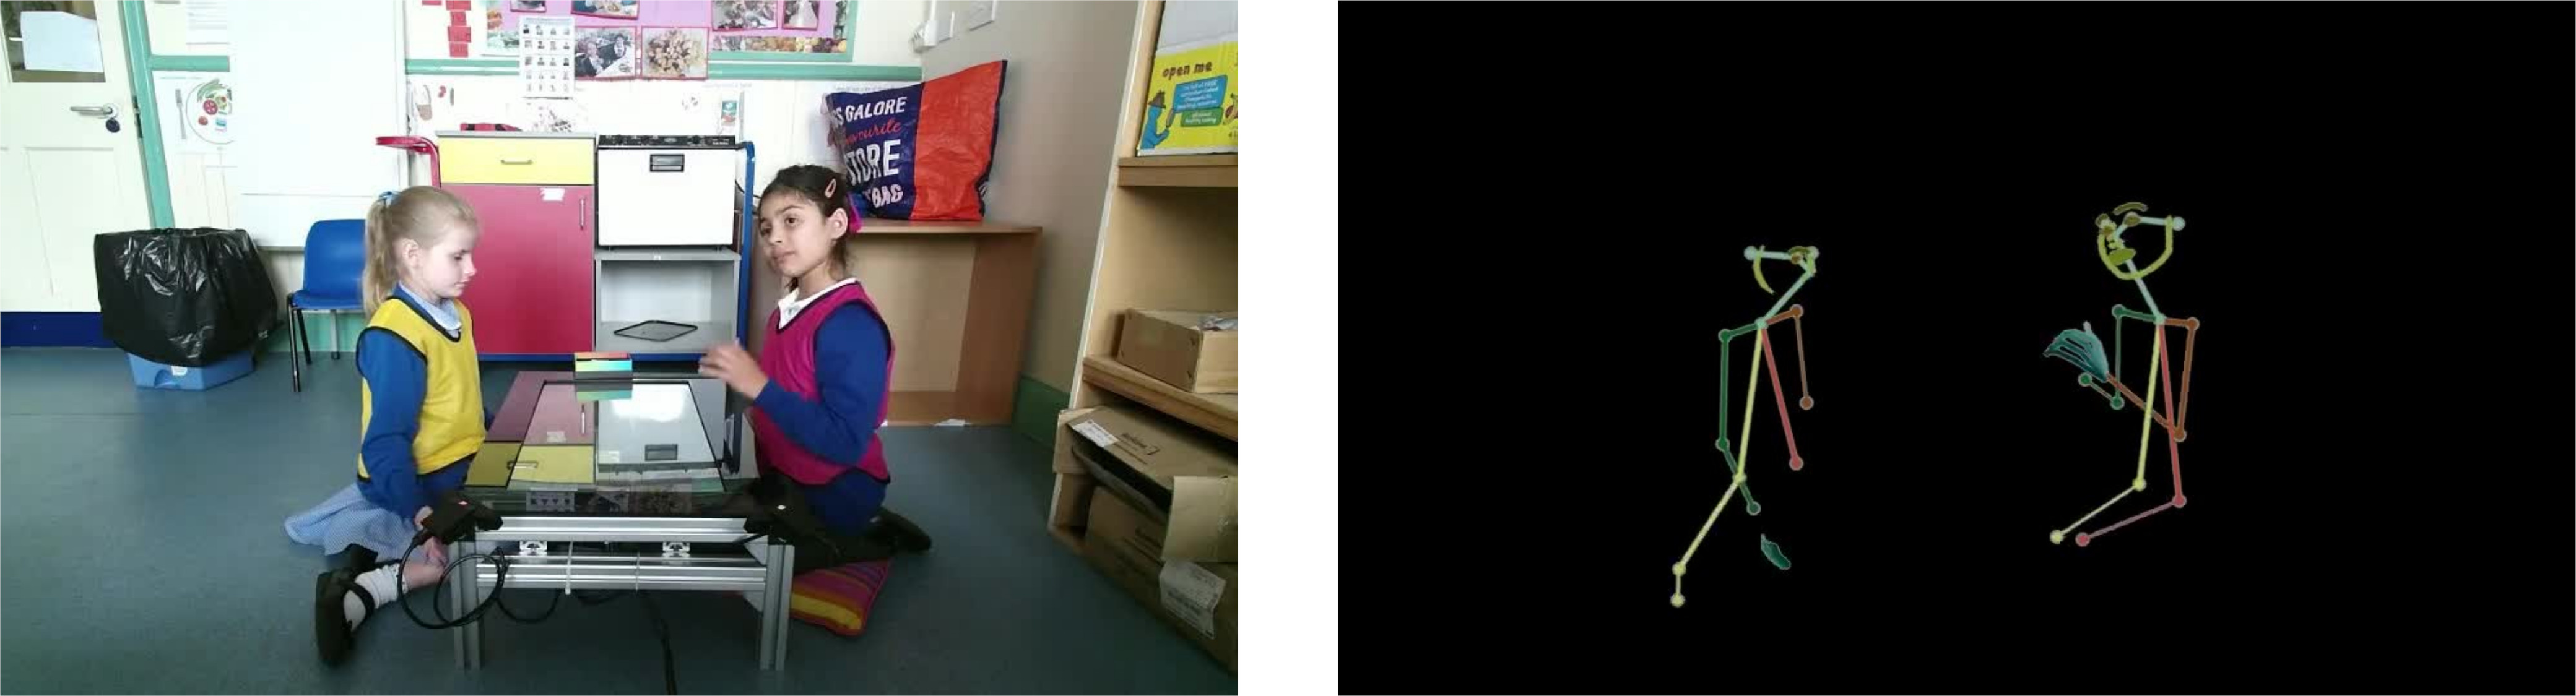
\includegraphics[width=0.9\linewidth]{kinematics_social_dynamics/clips.jpg}

    \textbf{Interaction imbalance}
    
    \textbf{Interaction valence}
    
    \textbf{Engagement}

    \badge[caption=Maddy Bartlett]{colleagues/maddy}
\end{frame}

\begin{frame}{Mean EFA projection of clips per social situation}

    \only<1>{
        The 20 clips were labelled after their salient social features
        (\emph{aggressive}, \emph{excited}, \emph{aimless}, \emph{fun},
        \emph{cooperative}, \emph{bored}, \emph{dominant}).

        \vspace{2cm}
        What happen if we project the ratings for 'aggressive' clips,
        'excited' clips, etc. onto the 3 EFA factors?

    }

    \only<2->{
    \begin{center}
        \includegraphics<2>[width=\linewidth]{kinematics_social_dynamics/means-imbalance-vs-valence.png}
        \includegraphics<3>[width=\linewidth]{kinematics_social_dynamics/means-imbalance-vs-engagement.png}
    \end{center}
    }

\end{frame}
}


\begin{frame}{Online games \& social datasets}

    \begin{center}
        %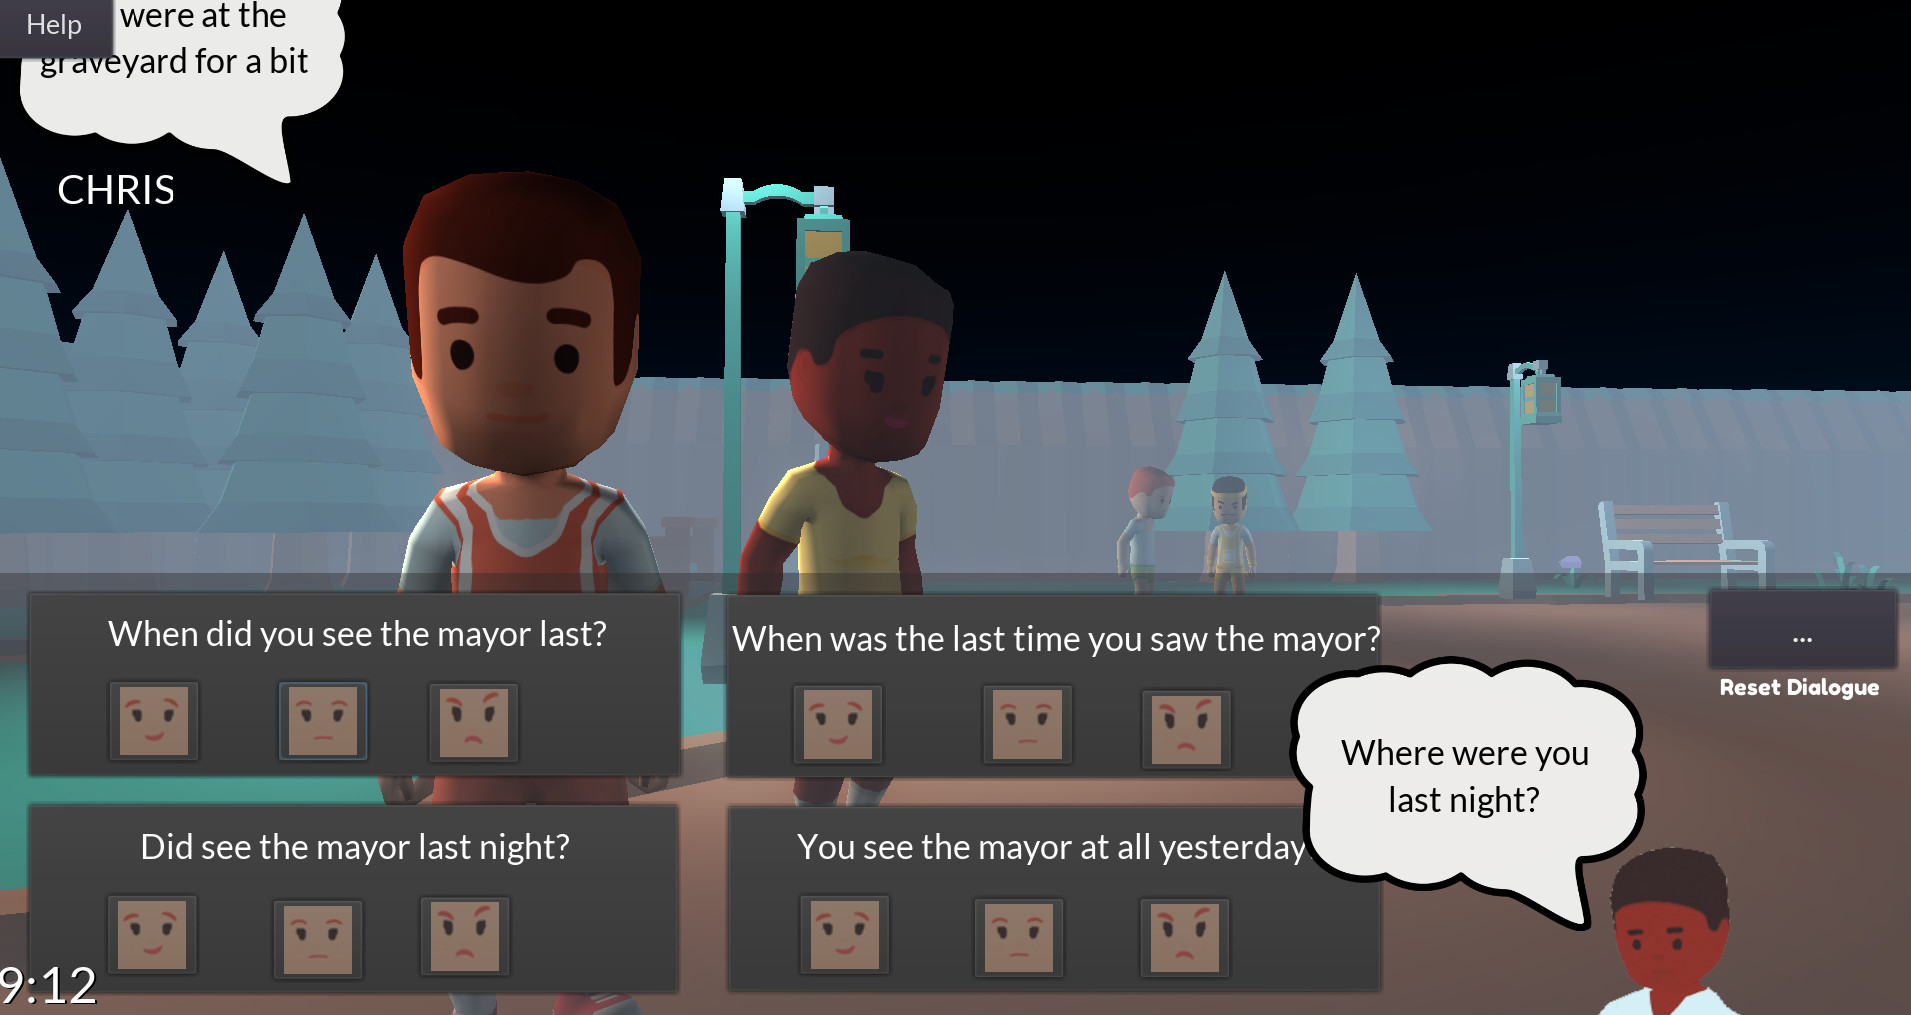
\includegraphics[width=0.6\linewidth]{figs/online-game/graveyard-detective-screenshot.jpg}
        \video[0.56]{0.45\linewidth}{figs/online-game/social-interaction-game.mp4?autostart}
        \begin{tikzpicture}
            \node at (0,0) {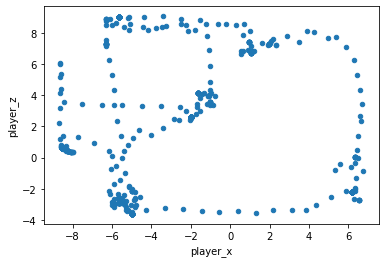
\includegraphics[width=0.3\linewidth]{figs/online-game/trajectory.png}};
           \node[anchor=north] at (1.5,1) {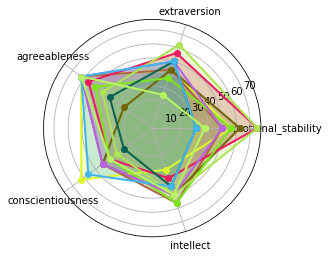
\includegraphics[width=0.3\linewidth]{figs/online-game/personality.png}};
        \end{tikzpicture}

    \end{center}

    \begin{center}
        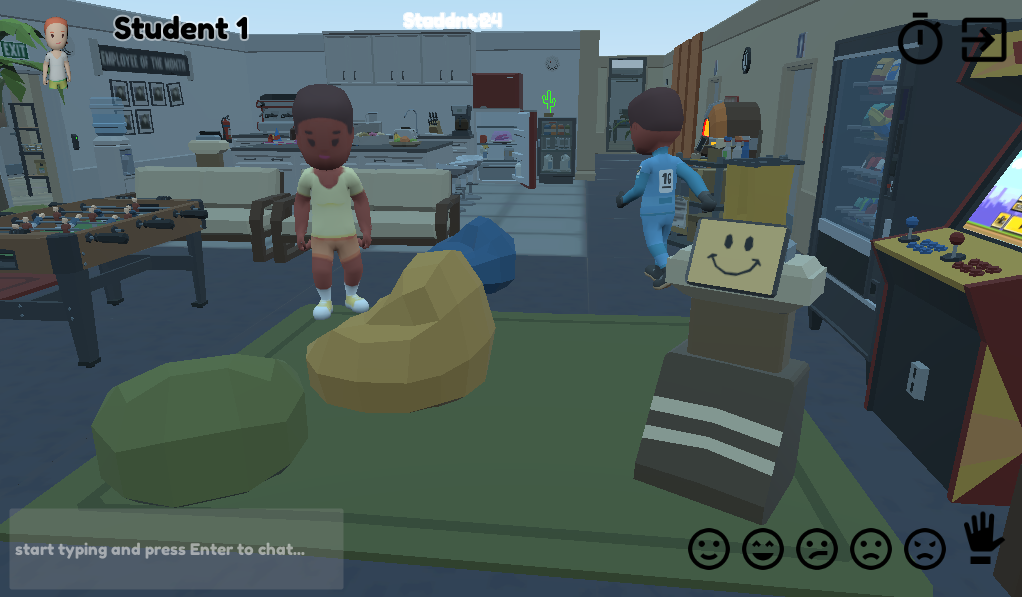
\includegraphics[width=0.45\linewidth]{figs/online-game/officebots-screenshot-2.png}
        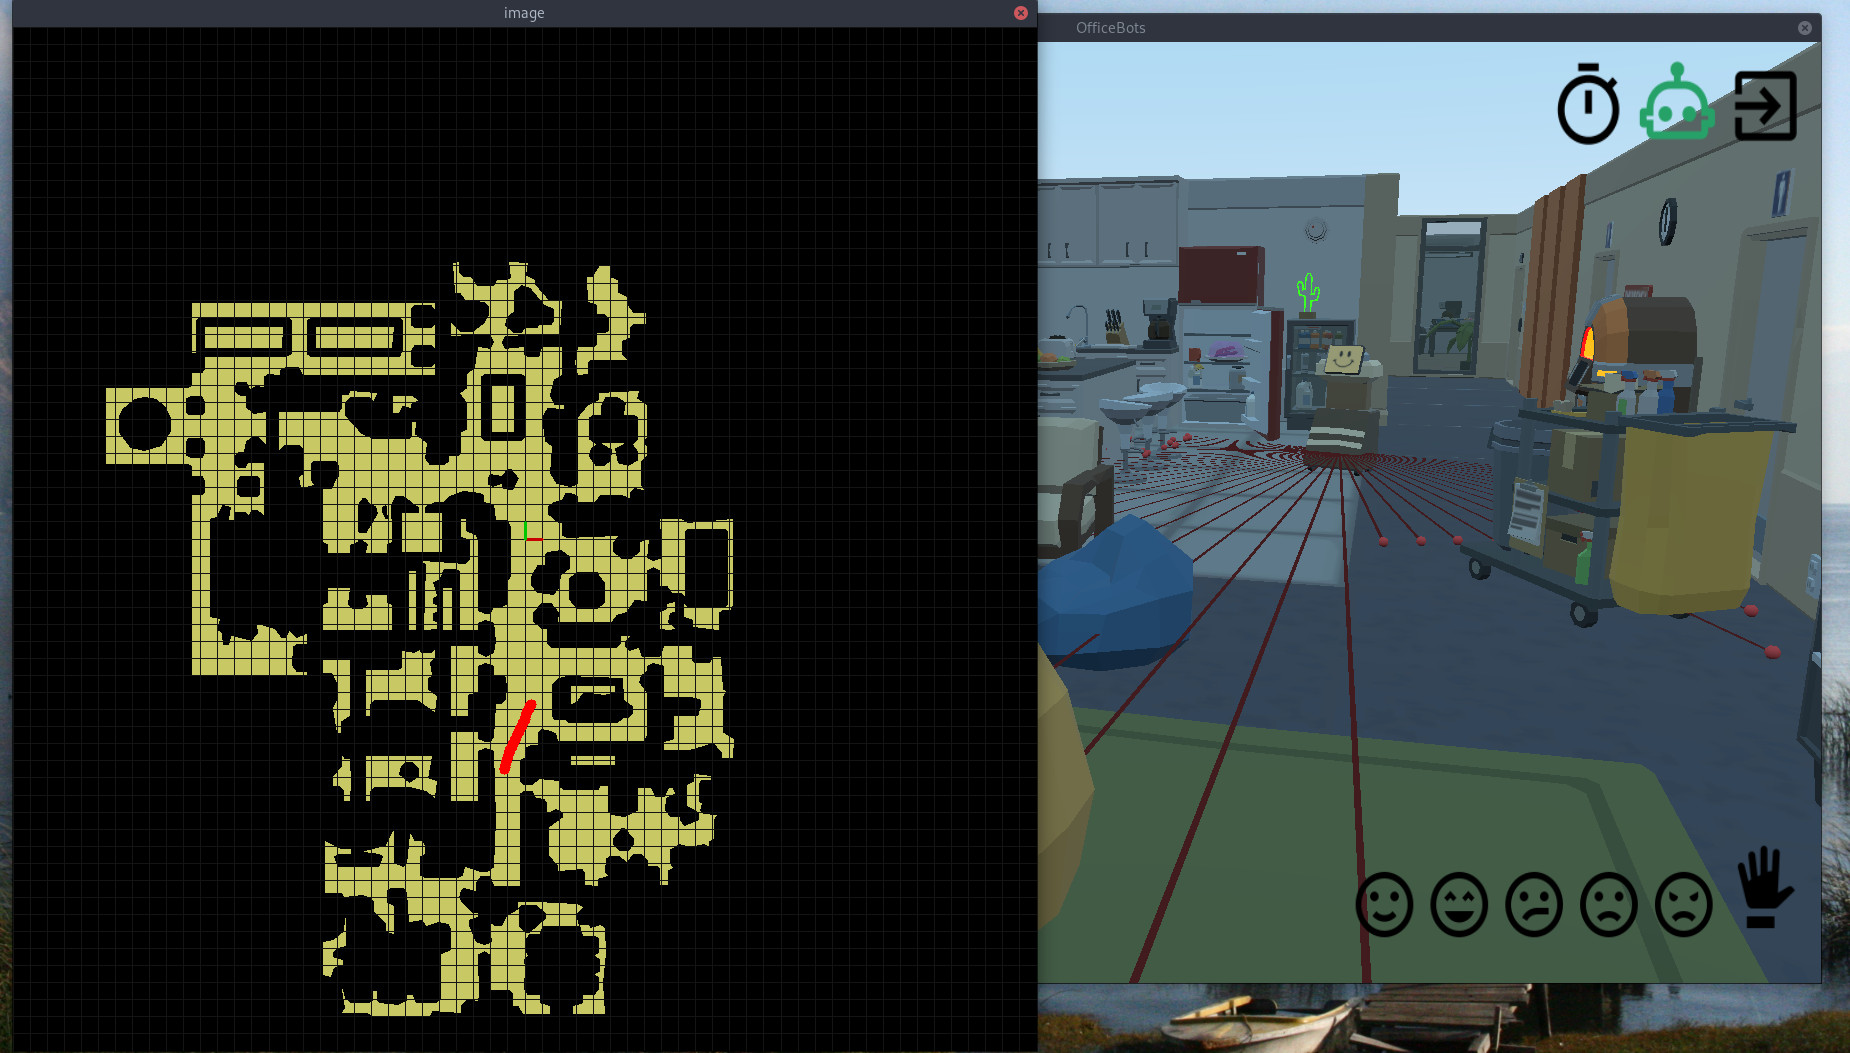
\includegraphics[width=0.45\linewidth]{figs/online-game/officebots-map.jpg}
    \end{center}


    \badge[caption=Nicola Webb]{colleagues/nicola}

\end{frame}




\section[Social policy learning]{...to in-situ social policy learning}


%\imageframe[caption={\textbf{Interactive Reinforcement Learning} to the rescue?}, color=black]{sparc/sophies}


\begin{frame}{Let set ourselves a challenge}

    Design \& run a study with:
    
    \begin{itemize}
        \item<+-> a real robot
        \item<+-> a real interaction (...with a human!)
        \item<+-> a continuous interaction
        \item<+-> a realistic task (large state vector \& action space)
        \item<+-> also including social behaviours \& social dynamics
        \item<+-> ...and of course, the robot should be autonomous
    \end{itemize}

\end{frame}

{
    \paper{Senft et al. \textbf{Teaching robots social autonomy from in situ
    human guidance} Science Robotics 2019}

\begin{frame}{IRL applied to social robotics}

    \begin{columns}
        \begin{column}{0.5\linewidth}

            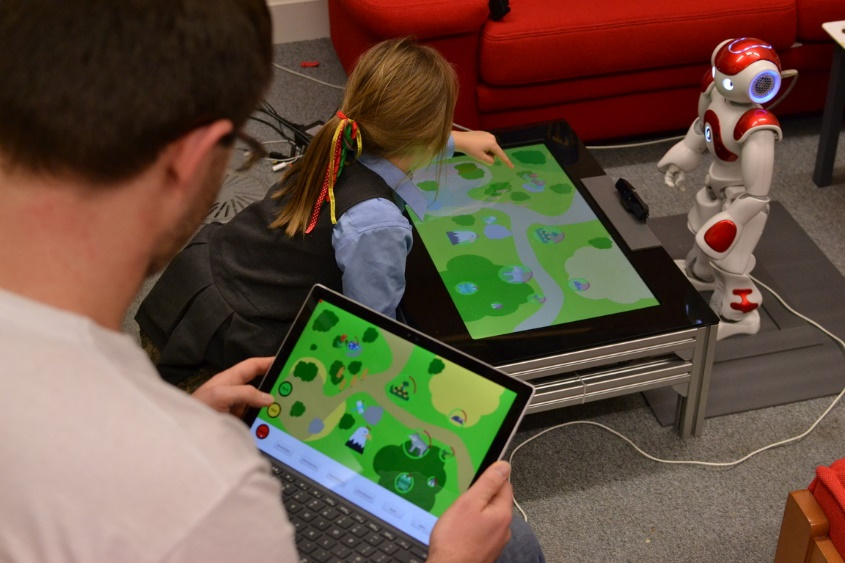
\includegraphics[width=\linewidth]{sparc/overview}

        \end{column}
        \begin{column}{0.5\linewidth}
            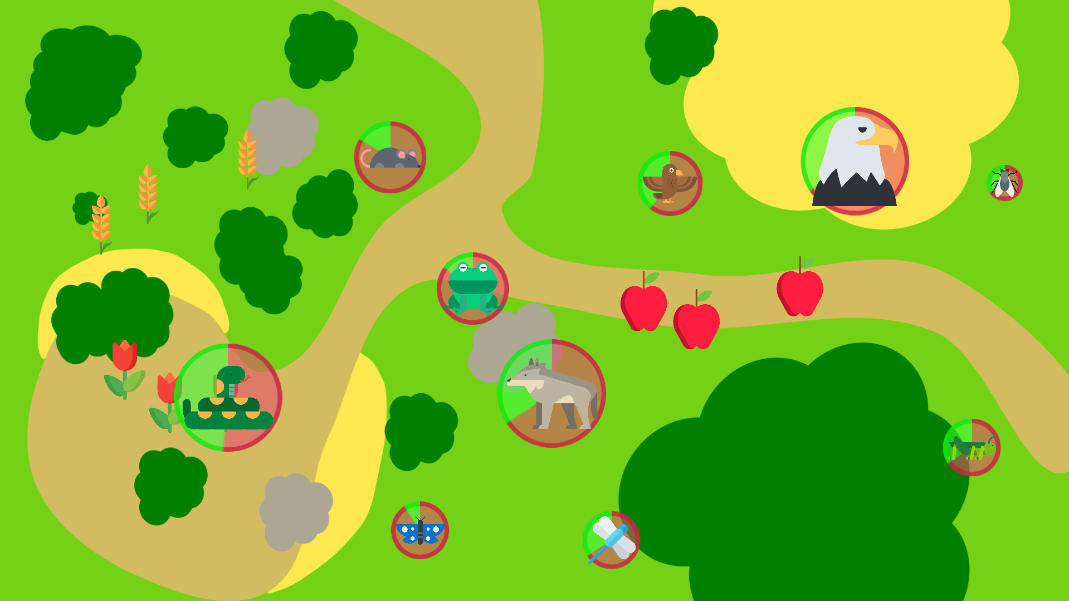
\includegraphics[width=\linewidth]{sparc/gui}
        \end{column}
    \end{columns}

    The children plays a game about food chains; the robot learns to guide them
    (\emph{task-specific action policy}) and encourage them (\emph{social action
    policy})

    Complex problem: 
    $|state| = 210$ $| action\_space| = 655$

    \badge[caption=Emmanuel Senft]{colleagues/emmanuel}
\end{frame}

\videoframe[0.56]{figs/sparc/video.mp4?noaudio&autostart}

\begin{frame}{Teacher's interface}
    \begin{center}
        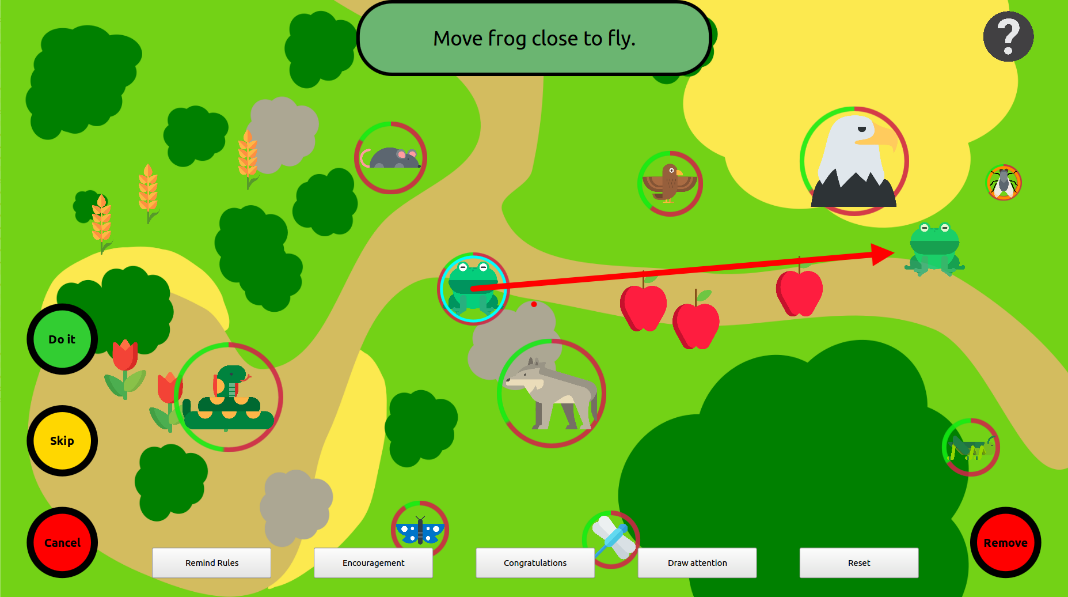
\includegraphics[width=0.9\linewidth]{sparc/woz-gui}
    \end{center}

    The robot's teacher (an end-user: might be the actual child's teacher) has a
    tablet interface that mirror's the child one, and add robot's teleoperation
    and rewards.

    \badge[caption=Emmanuel Senft]{colleagues/emmanuel}
\end{frame}


%\begin{frame}{Software architecture}
%    \begin{center}
%        \includegraphics[width=\linewidth]{figs/sparc/architecture}
%    \end{center}
%    \badge[caption=Emmanuel Senft]{colleagues/emmanuel}
%\end{frame}

%\imageframe[caption={Overall performance (pre-, mid-, post-test)},scale=0.9]{sparc/perf}

\begin{frame}{Learnt robot's behaviour}
    \only<1-2>{
        Distribution of actions for the 25 children participants:
    }
    \includegraphics<1>[width=0.9\linewidth]{sparc/actions-supervised}
    \includegraphics<2>[width=0.9\linewidth]{sparc/actions}

    \only<2>{
        $\rightarrow$ the robot personalises its action policies to the child's
        behaviour.
    }


    \only<3>{
        Time between a child's successful action and a praise:

        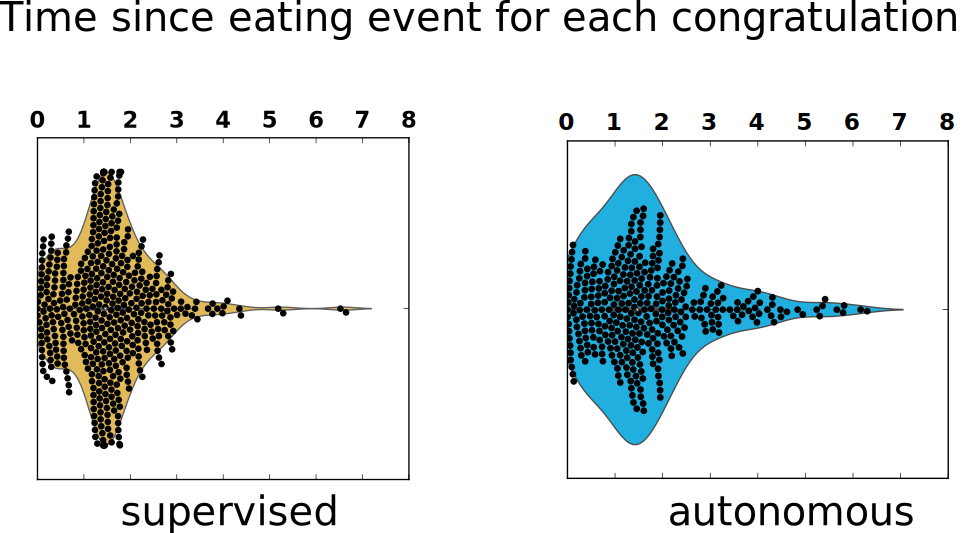
\includegraphics[width=0.9\linewidth]{sparc/social-timing}

        $\rightarrow$ the robot has also learnt an appropriate social timing.
    }

    \badge[caption=Emmanuel Senft]{colleagues/emmanuel}
\end{frame}
}


%\imageframe[color=black,caption={$|state| = 210$ $| action\_space| = 655$}]{sparc/gui}
%\imageframe[color=black]{sparc/overview}
%\videoframe[0.56]{figs/sparc/video.mp4}
%\imageframe[color=black]{sparc/woz-gui}
%\imageframe[caption={Overall performance (pre-, mid-, post-test)},scale=0.9]{sparc/perf}
%\imageframe[scale=0.9]{sparc/actions-supervised}
%\imageframe[scale=0.9]{sparc/actions}
%\imageframe[scale=0.9]{sparc/social-timing}

\begin{frame}{What does that means for the expert/teacher/end-user?}

    \begin{columns}
        \begin{column}{0.45\linewidth}
            
            \begin{center}
                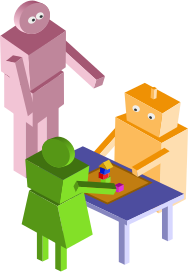
\includegraphics[width=0.9\linewidth]{sparc/sparc}
            \end{center}
        \end{column}
        \begin{column}{0.55\linewidth}
            \only<1>{
            \begin{itemize}
                \item {\bf Progressively transferring autonomy}  demonstrably
                    works in non-trivial tutoring scenarios

                \item (it also learns some elements of {\bf social behaviours} and
                    {\bf social timing})
            \end{itemize}
        }
            \only<2>{
                Key properties:

            \begin{itemize}
                \item \textbf{progressive autonomy} yet
                    \textbf{transparency} of the behaviour;
                \item \textbf{observability} and possibility to \textbf{take
                    over};
                \item because the training takes place in-situ, the
                    robot behaviours are \textbf{co-constructed} by the
                    teacher and the child
            \end{itemize}
        }
            \only<3>{
                Yet:

            \begin{itemize}
                \item Design of the input state tricky and largely task
                    dependent;
                \item What about more complex social behaviours?
                \item Would that sustain long-term interactions?
            \end{itemize}
            }
        \end{column}
    \end{columns}


\end{frame}

{
    \paper{Winkle et al. \textbf{In-Situ Learning from a Domain Expert for Real World Socially Assistive Robot Deployment} RSS 2020}

\begin{frame}{Co-design for real-world, long-term interaction}

    \begin{center}
        \begin{tikzpicture}
            \node at (0,0) {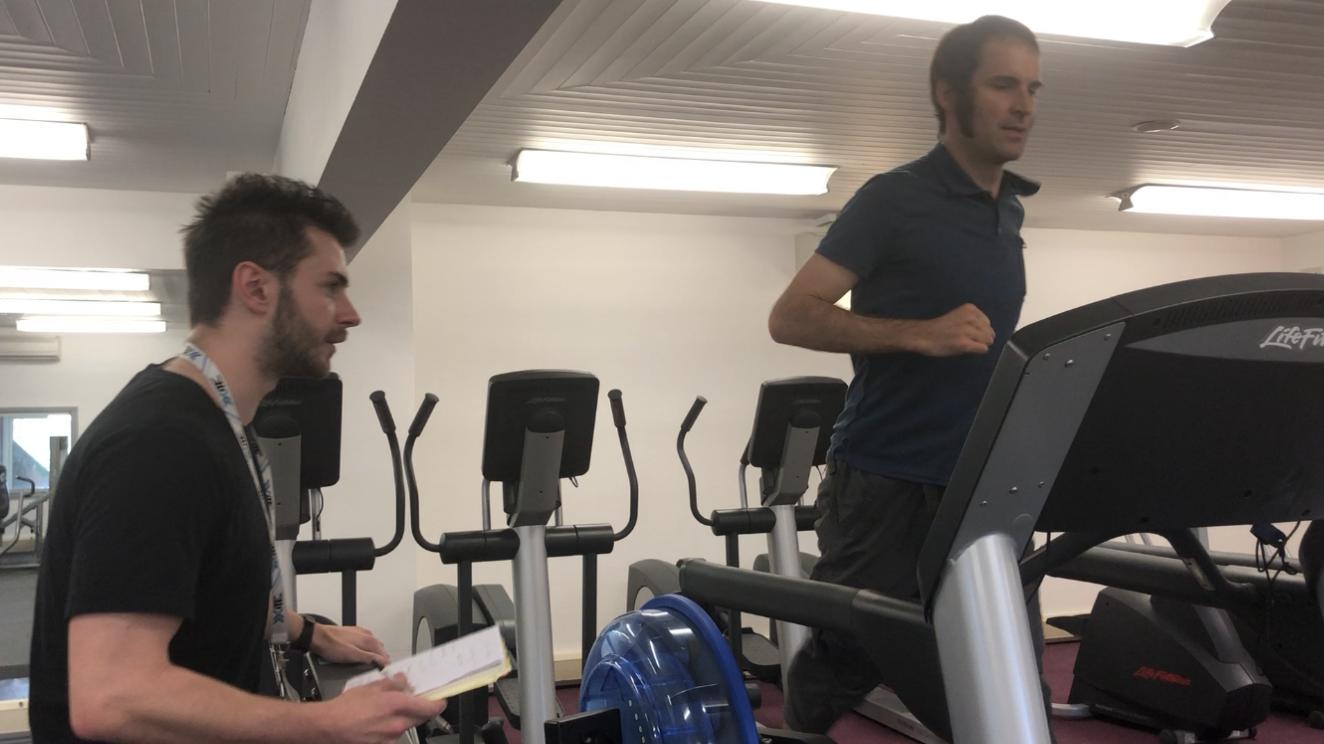
\includegraphics[width=0.6\linewidth]{figs/couch25k/couch25km-mock.jpg}};
           \node[anchor=north] at (4.5,-0.5) {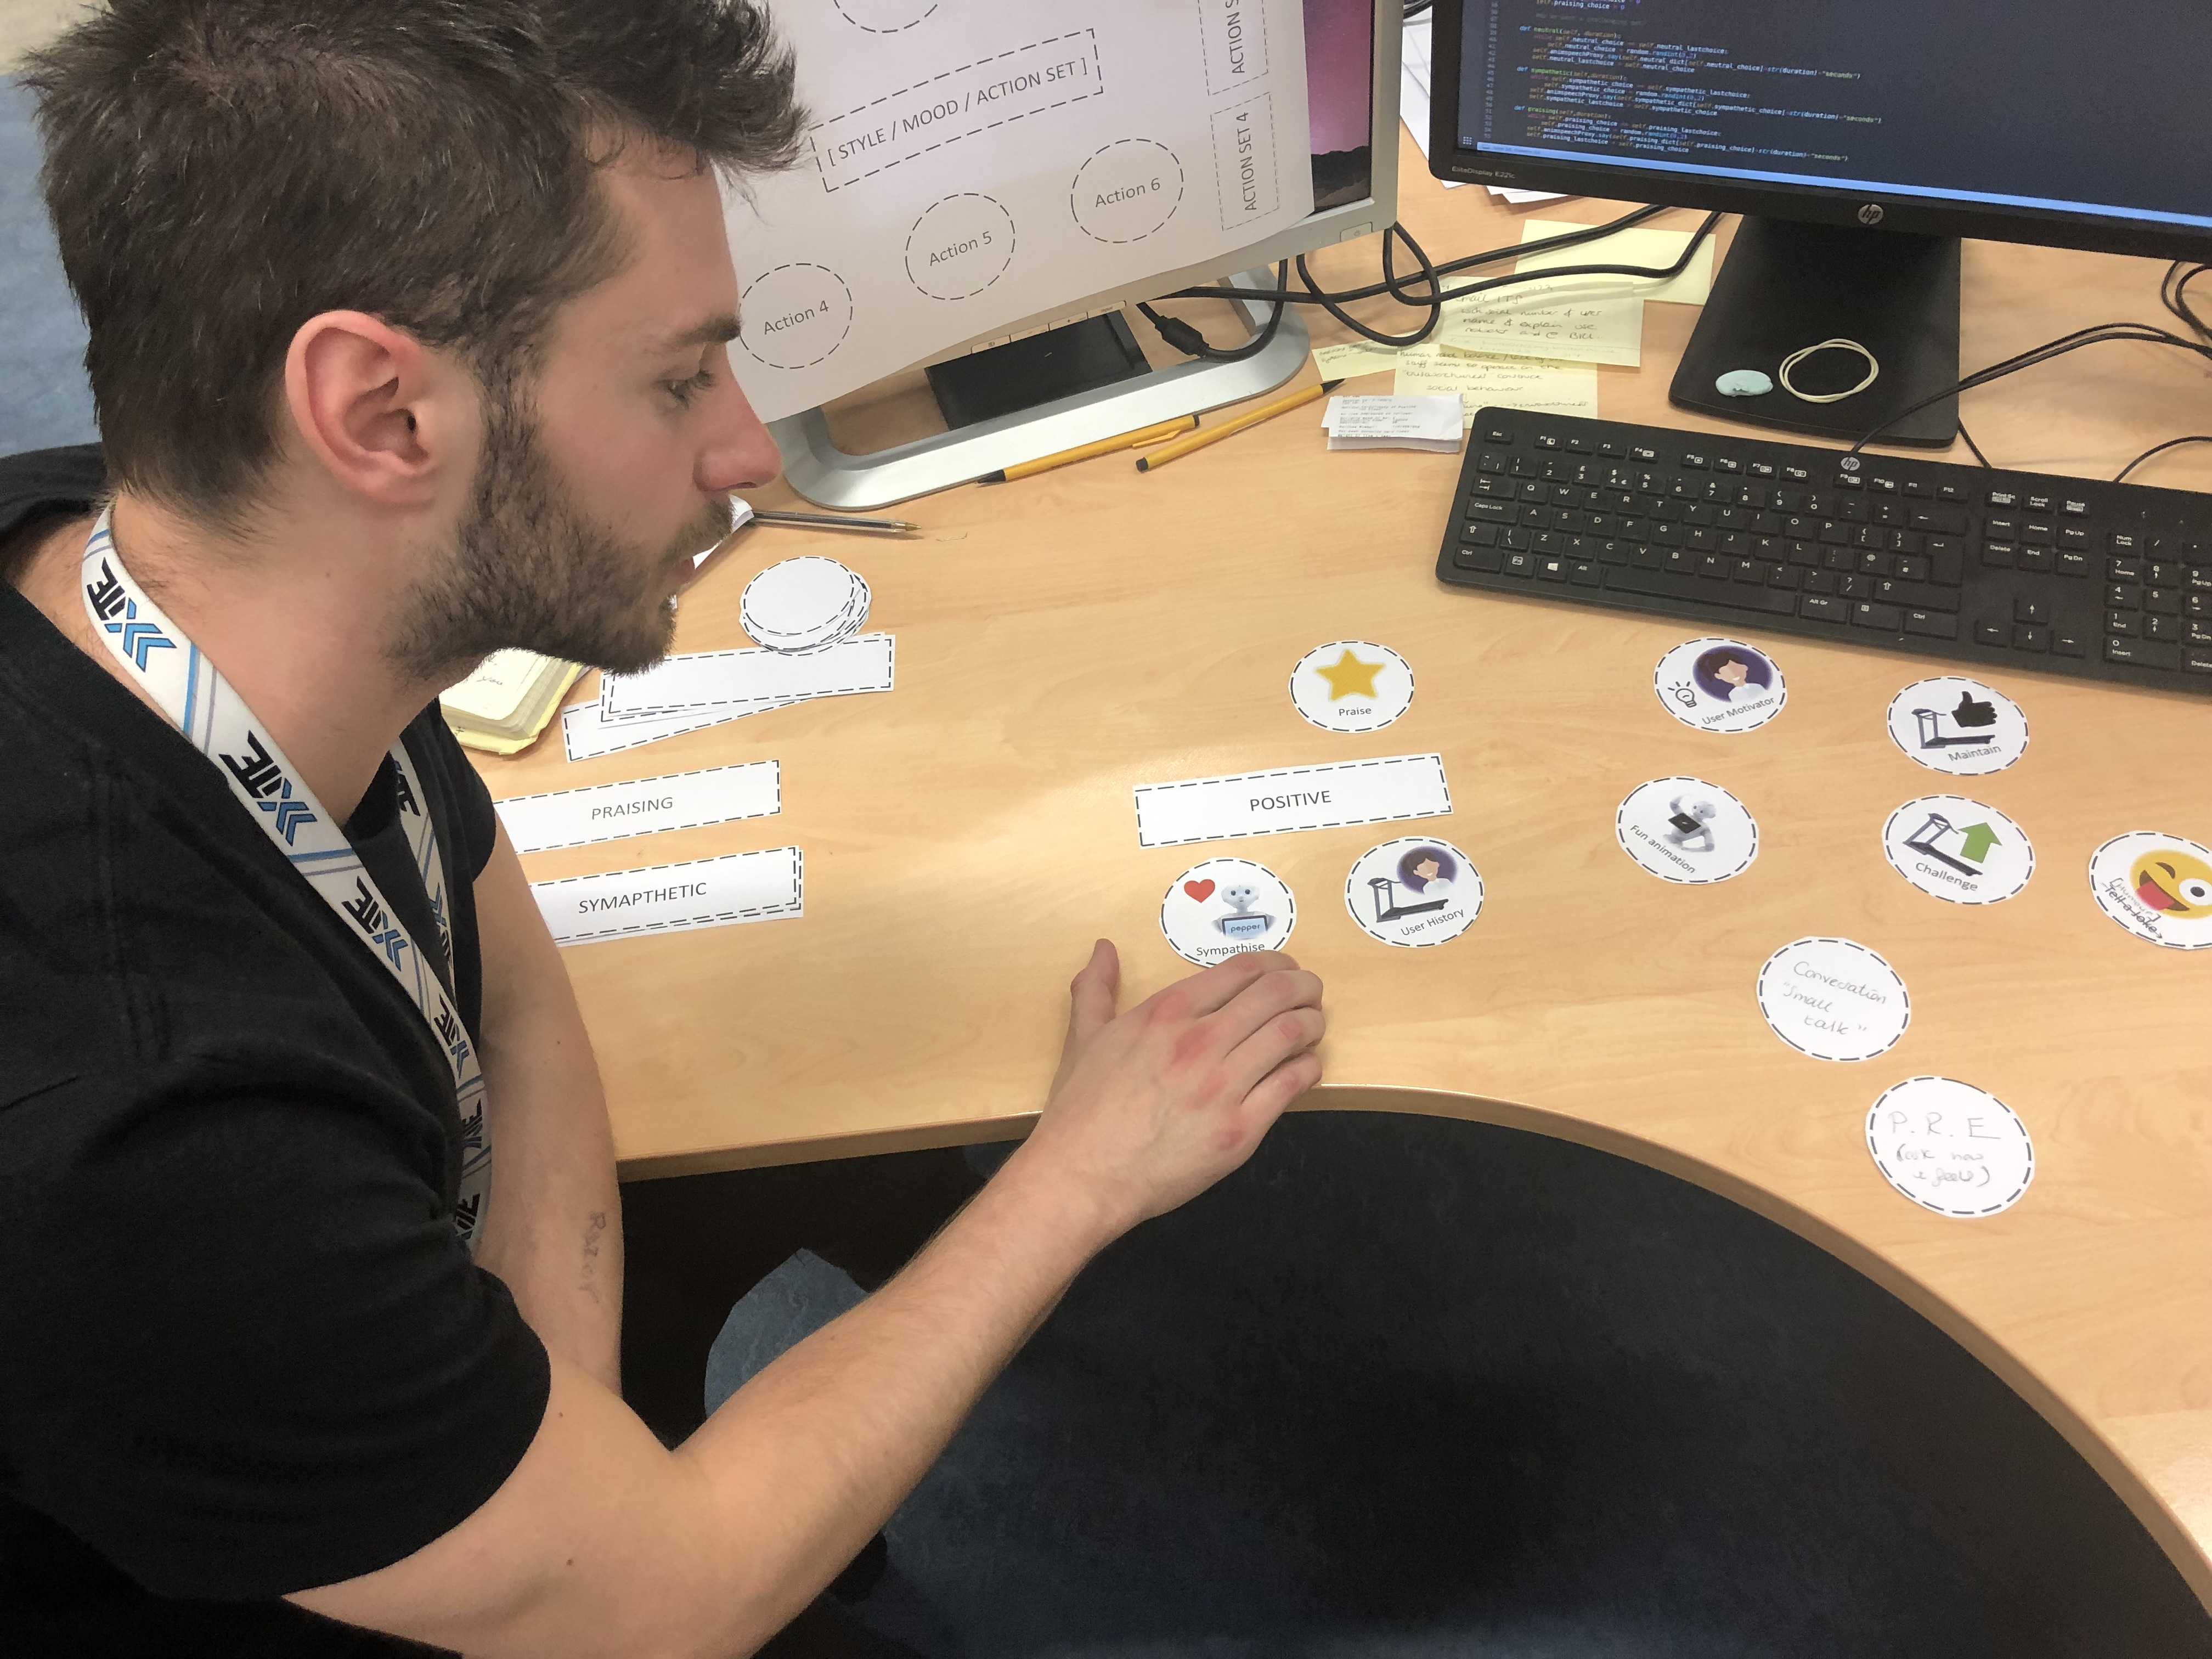
\includegraphics[trim=0 15cm 0 0,clip,width=0.6\linewidth]{figs/couch25k/codesign.jpg}};
        \end{tikzpicture}

    \end{center}
    \badge[caption=Katie Winkle]{colleagues/katie}
\end{frame}
}



{
    \paper{Winkle et al. \textbf{In-Situ Learning from a Domain Expert for Real World Socially Assistive Robot Deployment} RSS 2020}

\begin{frame}{Expert-in-the-loop machine learning}

    \vspace{0.2cm}

    \begin{columns}
        \begin{column}{0.5\linewidth}
                \centering
                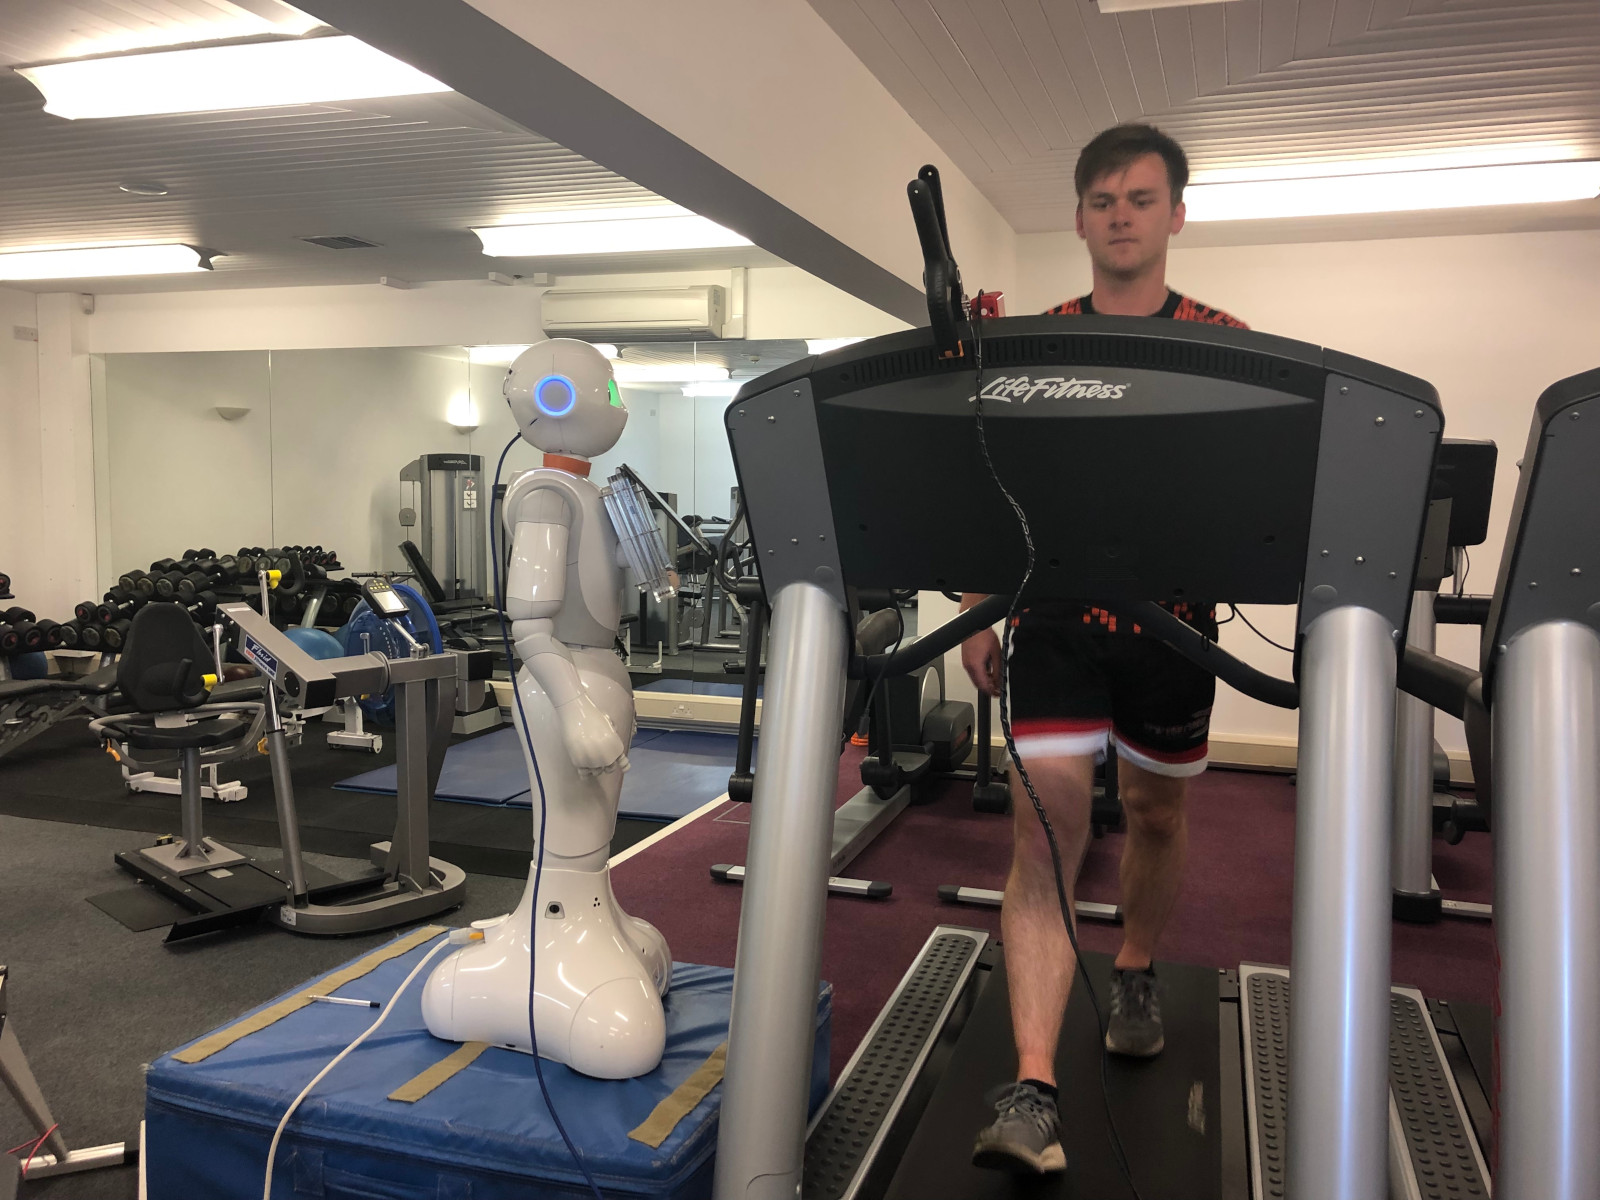
\includegraphics[height=3cm]{couch25k/hri.jpg}
        \end{column}
        \begin{column}{0.5\linewidth}
                \centering
                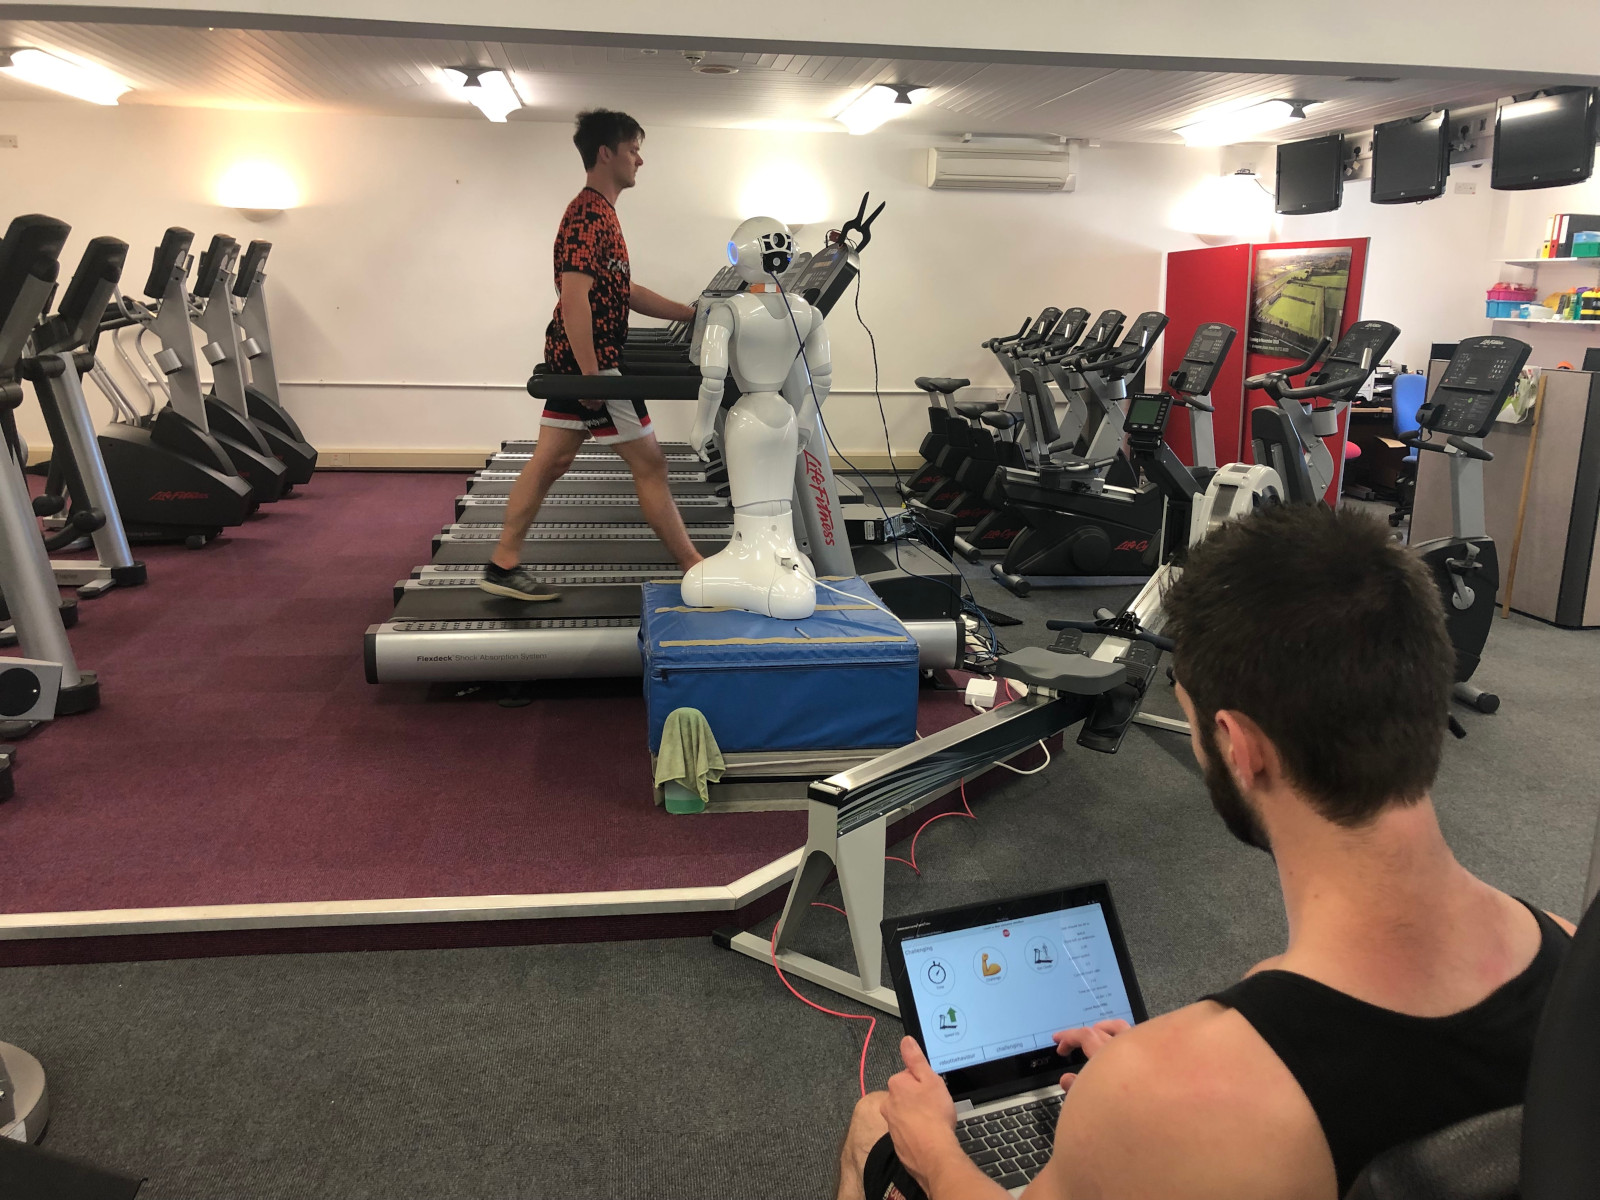
\includegraphics[height=3cm]{couch25k/supervised.jpg}
        \end{column}
    \end{columns}

        \centering
        \includegraphics[height=4cm]{couch25k/architecture.pdf}

    \badge[caption=Katie Winkle]{colleagues/katie}
\end{frame}
}

\begin{frame}{Couch to 5km study}
    \begin{itemize}
        \item 9 participants
        \item 3 months; 27 one-hour sessions per participants
        \item 20 input features; 11 actions (task-specific or social)
        \item human-in-loop design and machine learning
        \item robot evolving from full teleoperation to full task and social
            autonomy
    \end{itemize}

    \badge[caption=Katie Winkle]{colleagues/katie}
\end{frame}

{
    \paper{Winkle et al. \textbf{In-Situ Learning from a Domain Expert for Real World Socially Assistive Robot Deployment}
    RSS 2020}
    \begin{frame}{Learnt policies}
        \begin{center}
            \includegraphics<1>[width=\linewidth]{figs/couch25k/finalactiondist-no-autonomous.png}
            \includegraphics<2>[width=\linewidth]{figs/couch25k/finalactiondist.png}
            \includegraphics<3>[width=\linewidth]{figs/couch25k/fullcomp_lbmr.pdf}
        \end{center}
\end{frame}
}

\section[Generating behaviours]{Generating socially-congruent behaviours}

{
    \paper{Wallbridge et al. \textbf{The Effectiveness of Dynamically Processed
    Incremental Descriptions in Human Robot Interaction} Transaction on HRI
    2021, to appear}

\begin{frame}{Dynamic vs non-ambiguous language}
    \begin{center}
        \only<1>{
        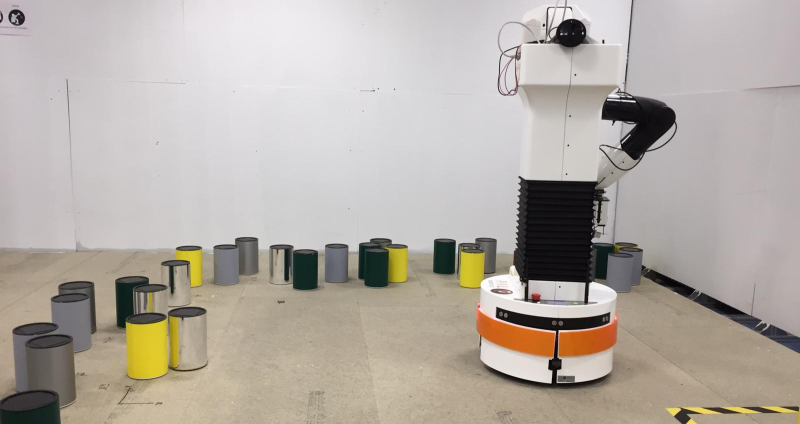
\includegraphics[width=0.8\linewidth]{dynamic-language/Preview_image}
        }

        \only<2>{
            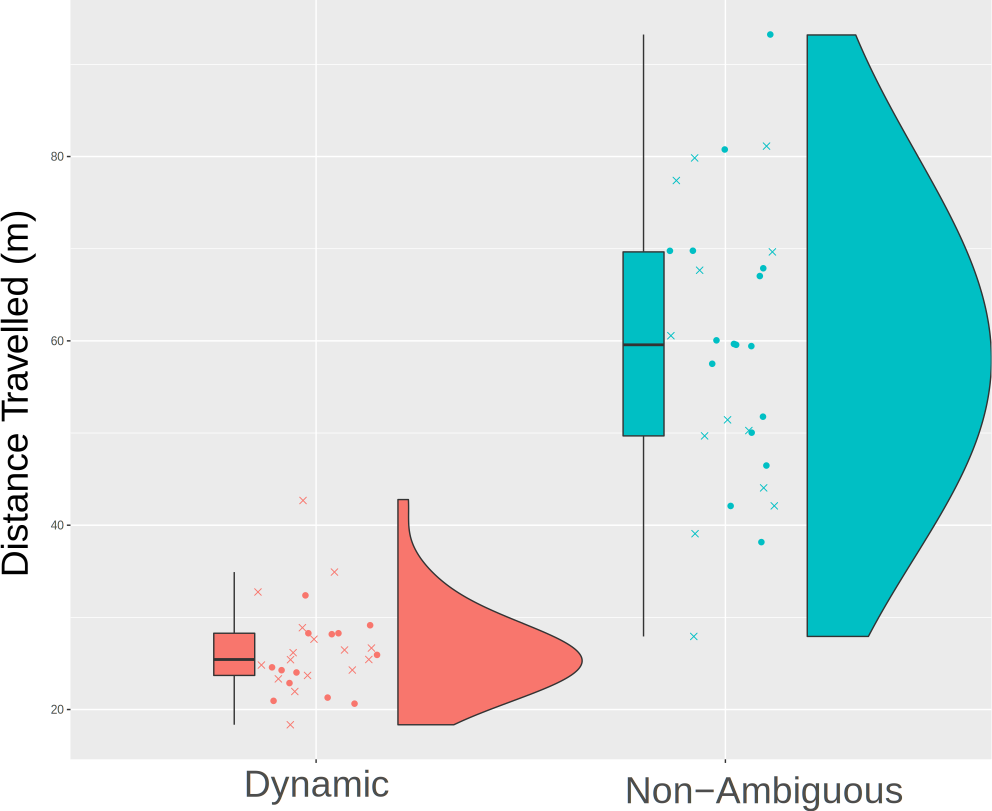
\includegraphics[width=0.45\linewidth]{dynamic-language/Dist_graph}
            \includegraphics[width=0.45\linewidth]{dynamic-language/Time_taken_Both}
        }

        {\scriptsize
        \textbf{Condition Non-ambiguous}: ``A grey barrel is next to a grey barrel, next to a silver barrel and
        next to a green barrel.''

        \textbf{Condition Dynamic}: ``Turn left about 90 degrees.''... ``Keep
        going''... ``Go forward''... ``The silver barrel next to the chrome
        barrel.''
        }


    \end{center}

    \badge[caption=Chris Wallbridge]{colleagues/chris}
\end{frame}
}

\begin{frame}{Expressive eyes}
    \begin{center}
        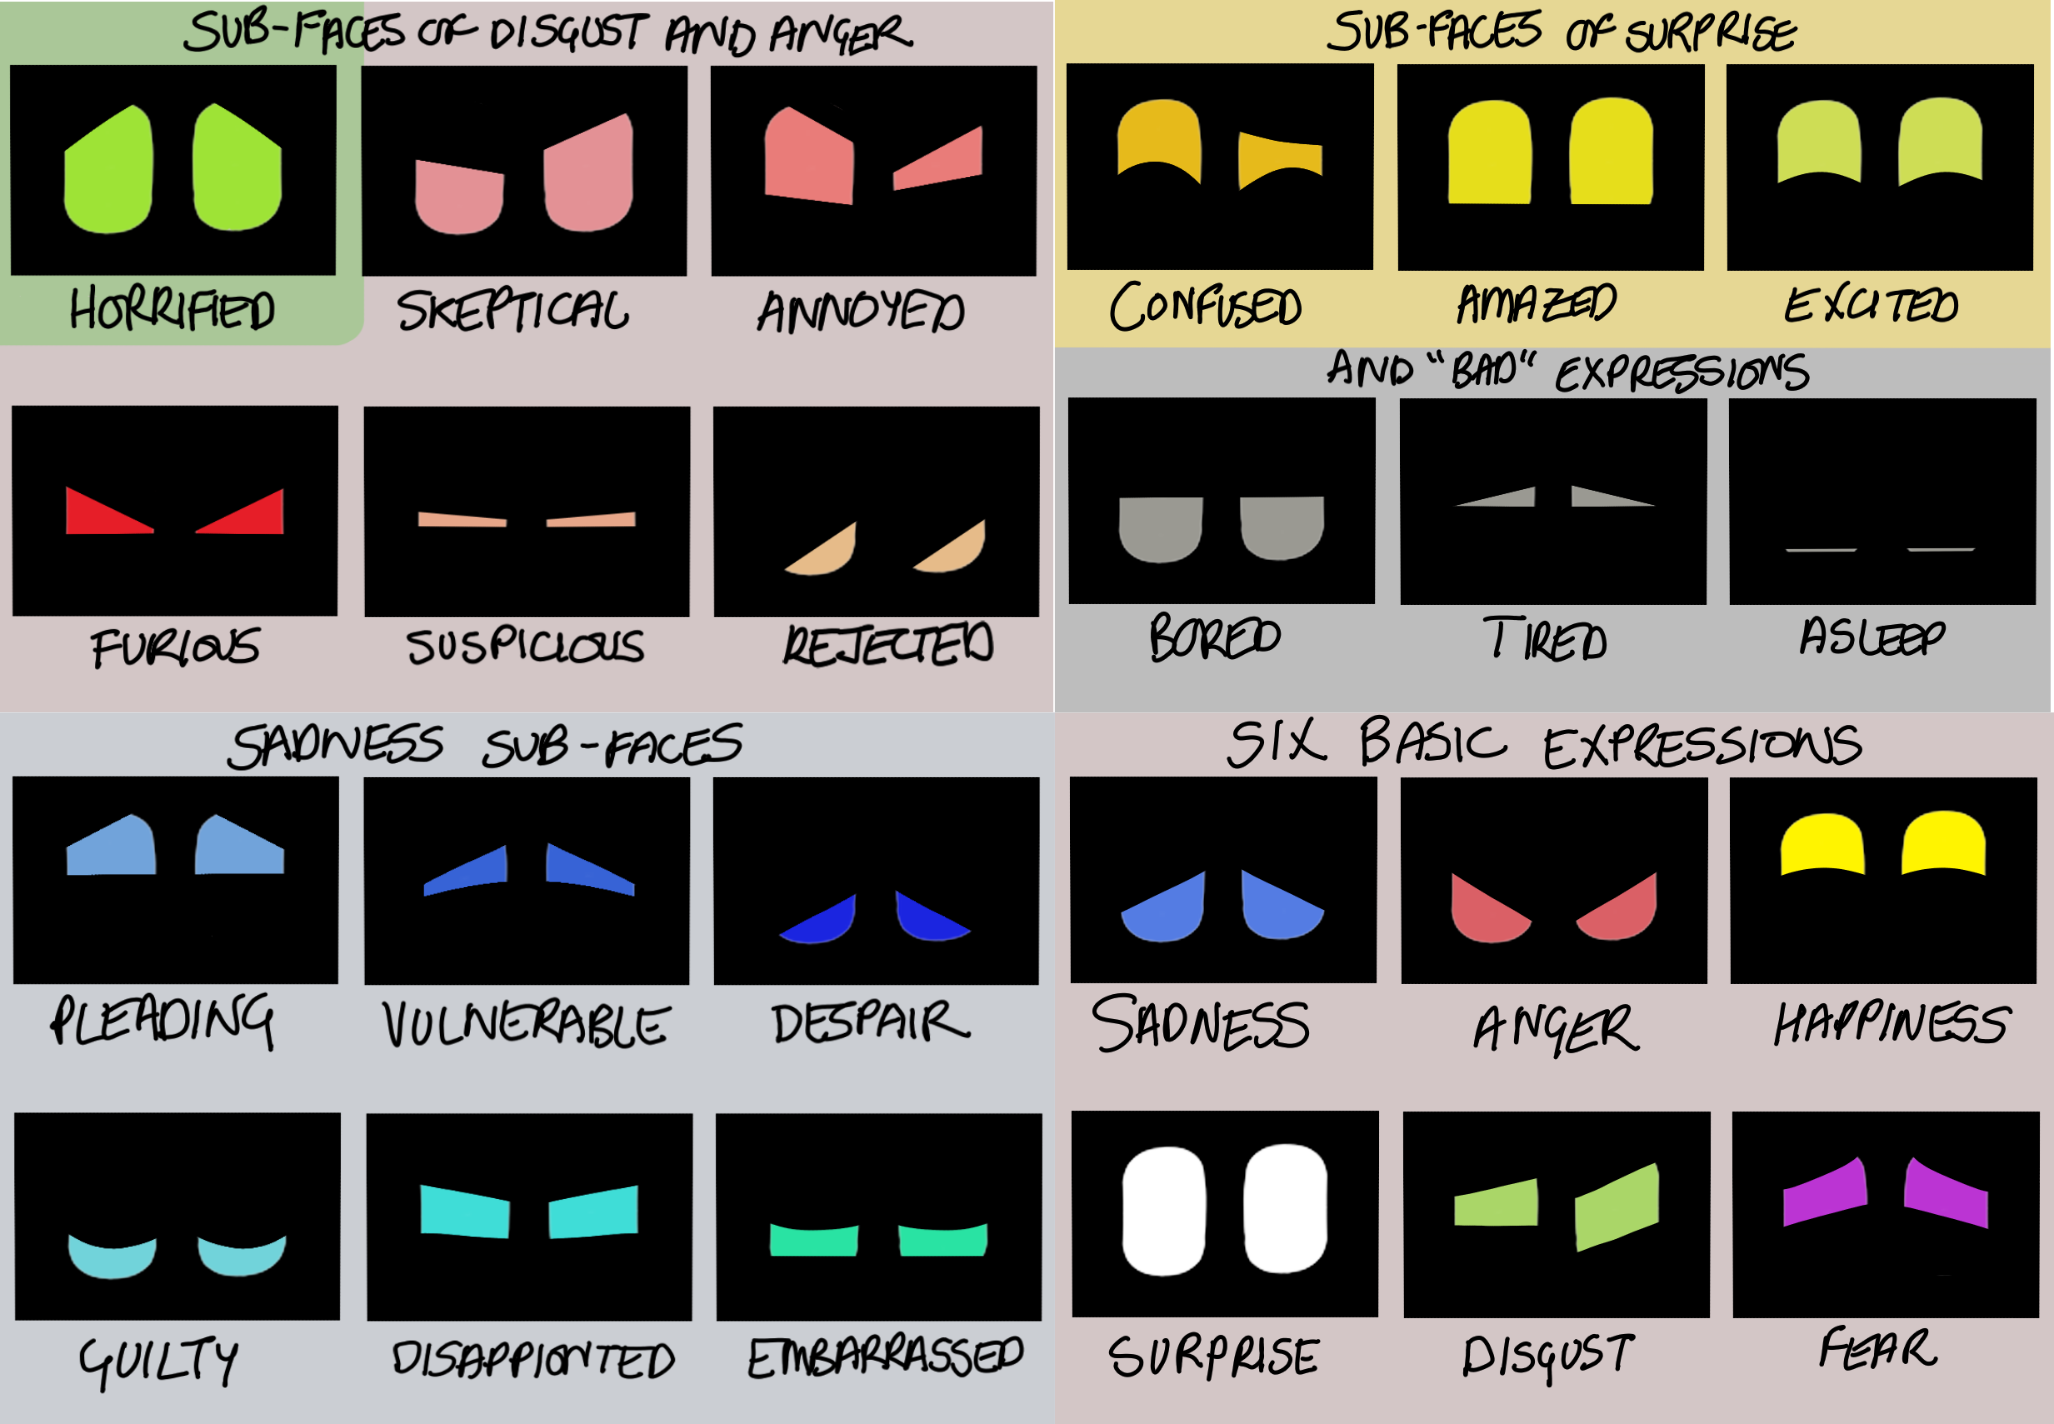
\includegraphics[width=0.45\linewidth]{figs/expressive-eyes/expressive-eyes-chambers.png}
        \hspace{0.5em}
        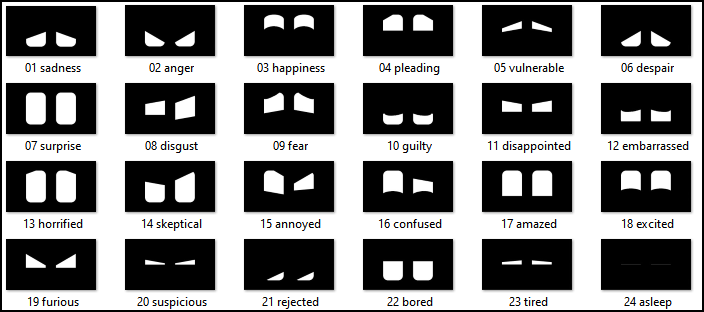
\includegraphics[width=0.45\linewidth]{figs/expressive-eyes/generated_faces.png}
    \end{center}

    \begin{columns}
        \begin{column}{0.5\linewidth}
            {
                \scriptsize
            \begin{itemize}
                \item inspired by Anki Cozmo/Vector
                \item expression interpretation validated online
                \item work by MSc student Catherine Chambers
                \item
                    \href{https://git.brl.ac.uk/s-lemaignan/expressive-eyes}{git.brl.ac.uk/s-lemaignan/expressive-eyes}
            \end{itemize}
        }
        \end{column}
        \begin{column}{0.5\linewidth}
        \begin{center}
            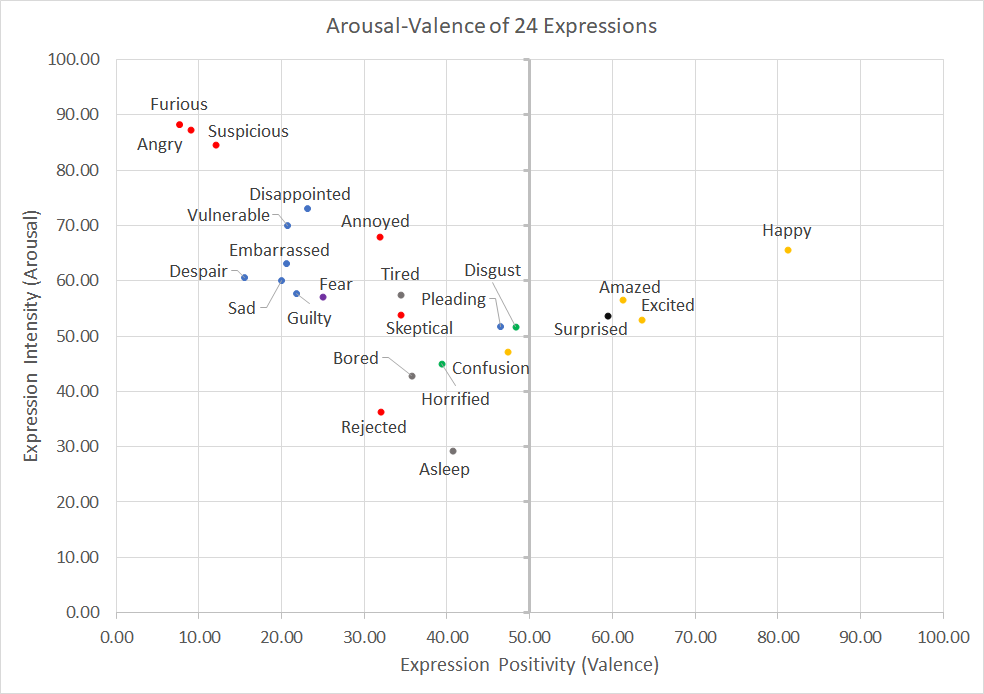
\includegraphics[width=\linewidth]{figs/expressive-eyes/online-study.png}
        \end{center}
        \end{column}
    \end{columns}
\end{frame}



%%%%%%%%%%%%%%%%%%%%%%%%%%%%%%%%%%%%%%%%%%%%%%%%%%%%%%%%%%%%%%%%%%%%%%%%%%%%%
%%%%%%%%%%%%%%%%%%%%%%%%%%%%%%%%%%%%%%%%%%%%%%%%%%%%%%%%%%%%%%%%%%%%%%%%%%%%%

\section{What next?}

\imageframe[scale=0.9]{figs/echos-big-picture}

%
%\begin{frame}[plain]
%    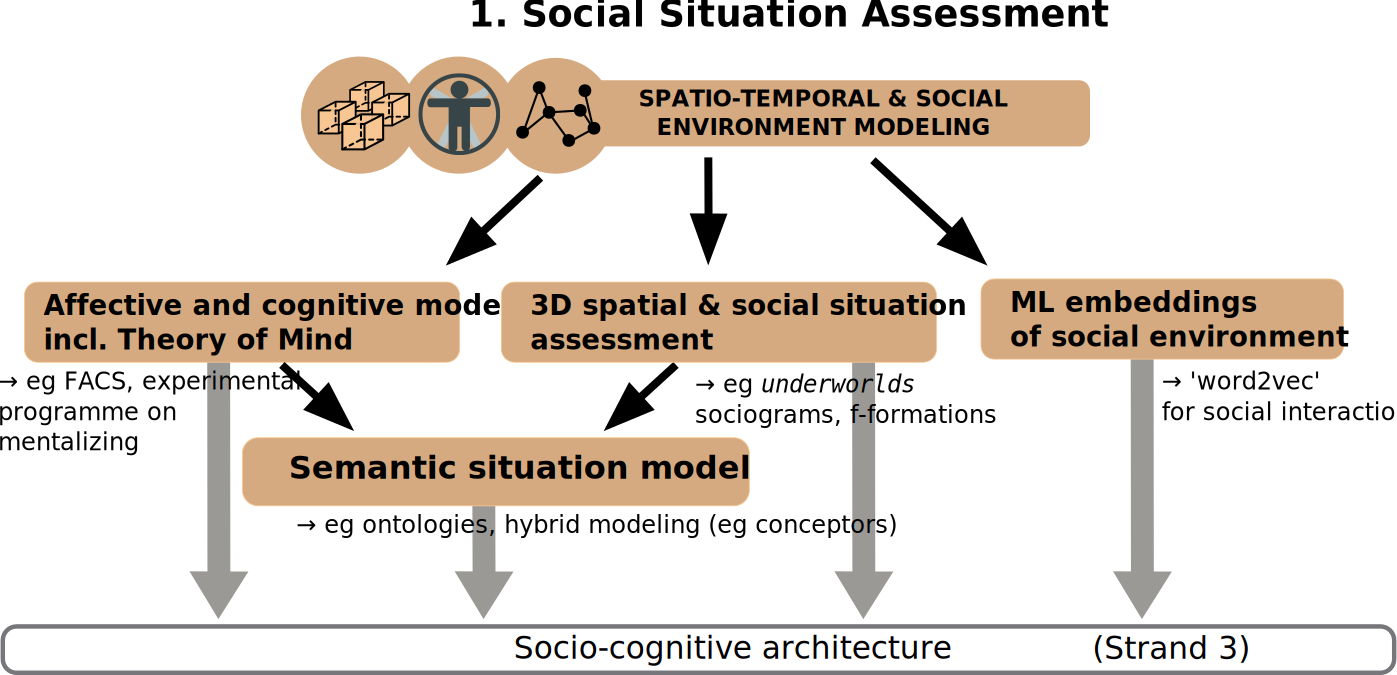
\includegraphics[width=\columnwidth]{architectures/strand1.pdf}
%
%    \vspace{1em}
%    \begin{columns}
%        \begin{column}{0.4\linewidth}
%        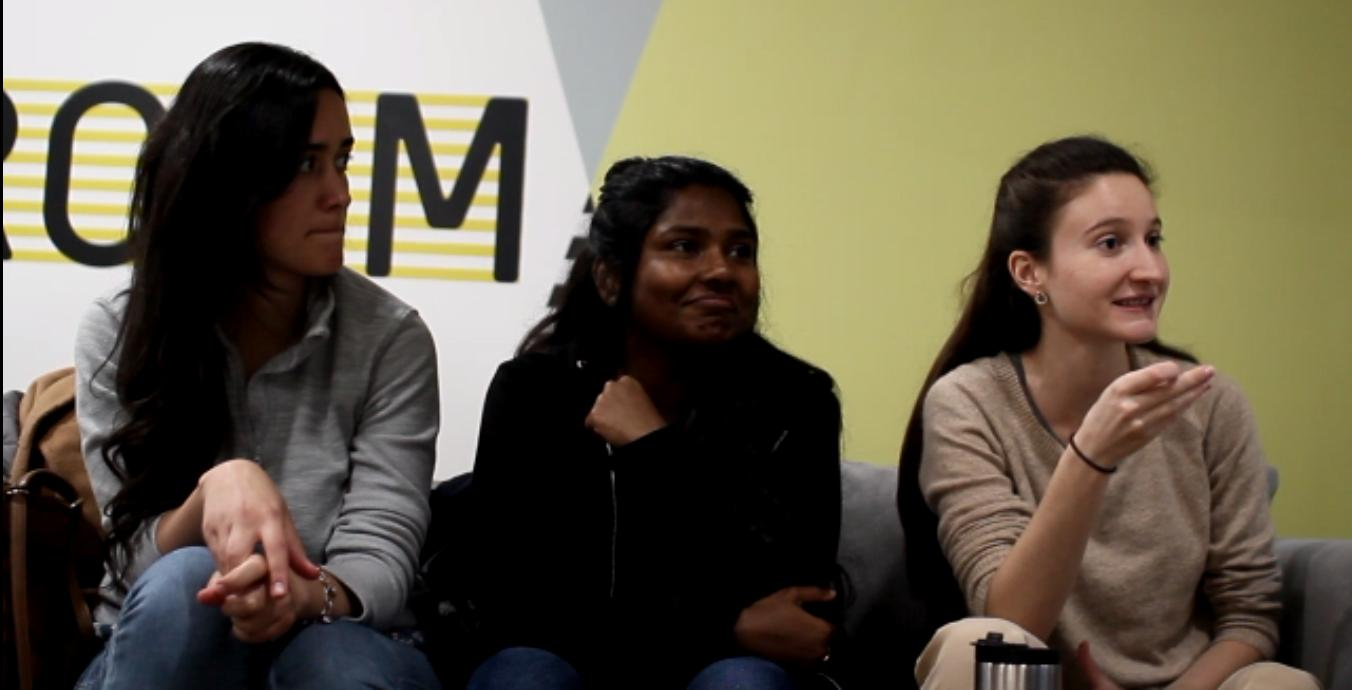
\includegraphics[width=\columnwidth]{social-interactions/social.jpg}
%
%        \end{column}
%        \begin{column}{0.7\linewidth}
%            \scriptsize
%            \begin{itemize}
%                \item SotA machine learning: \textbf{attention nets};
%                    \textbf{deep graph nets}
%                \item \textbf{Social embeddings}: learn an encoding of social
%                    interactions
%                \item \textbf{hybrid pipeline}: eg \emph{conceptors} to build symbolic
%                    models from neural nets 
%                \item real-world \textbf{robustness}: algorithmic redundancy; soft. eng.
%                    expertise (going beyond throw-away research code)
%            \end{itemize}
%
%        \end{column}
%    \end{columns}
%\end{frame}
%
%%\againframe<3>{wps}
%
%
%
%
%%\againframe<5>{wps}
%
%\begin{frame}<4>[plain]
%    \begin{center}
%    \begin{columns}
%        
%
%        \begin{column}{0.3\linewidth}
%            \includegraphics[height=0.75\paperheight]{croquignole-narrow.jpg}
%        \end{column}
%
%
%        \begin{column}{0.7\linewidth}
%            \centering
%            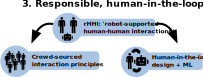
\includegraphics[width=\columnwidth]{architectures/strand4}
%            \vspace{1em}
%
%            \scriptsize
%            \begin{enumerate}
%                \item<1-> interactive reinforcement learning
%                    \begin{itemize}
%                        \item \emph{\scriptsize how to scale it to multiple tasks?}
%                        \item \emph{\scriptsize how to deal with non-trivial semantics?}
%                    \end{itemize}
%                \item<2-> intrinsic social motivation
%                    \begin{itemize}
%                        \item \scriptsize large-scale public engagement to
%                            \textbf{co-design interaction principles: meaningful \& useful social goals}
%                    \end{itemize}
%                \item<3-> responsible AI
%                    \begin{itemize}
%                        \item \scriptsize\textbf{crowd-sourcing social norms} for human-robot
%                            interactions
%                    \end{itemize}
%
%            \end{enumerate}
%            \vspace{1em}
%
%            \onslide<4>{
%            $\rightarrow$ shift from human-robot interactions to \textbf{robot-supported human-human interactions}
%            }
%
%
%        \end{column}
%
%
%    \end{columns}
%    \end{center}
%\end{frame}
%
%\againframe<4>{wps}

\begin{frame}{KEY SCIENTIFIC CHALLENGES}

    \begin{center}
    We want more real-world, long-term, autonomous interactions!

        %        \resizebox{\linewidth}{!}{
        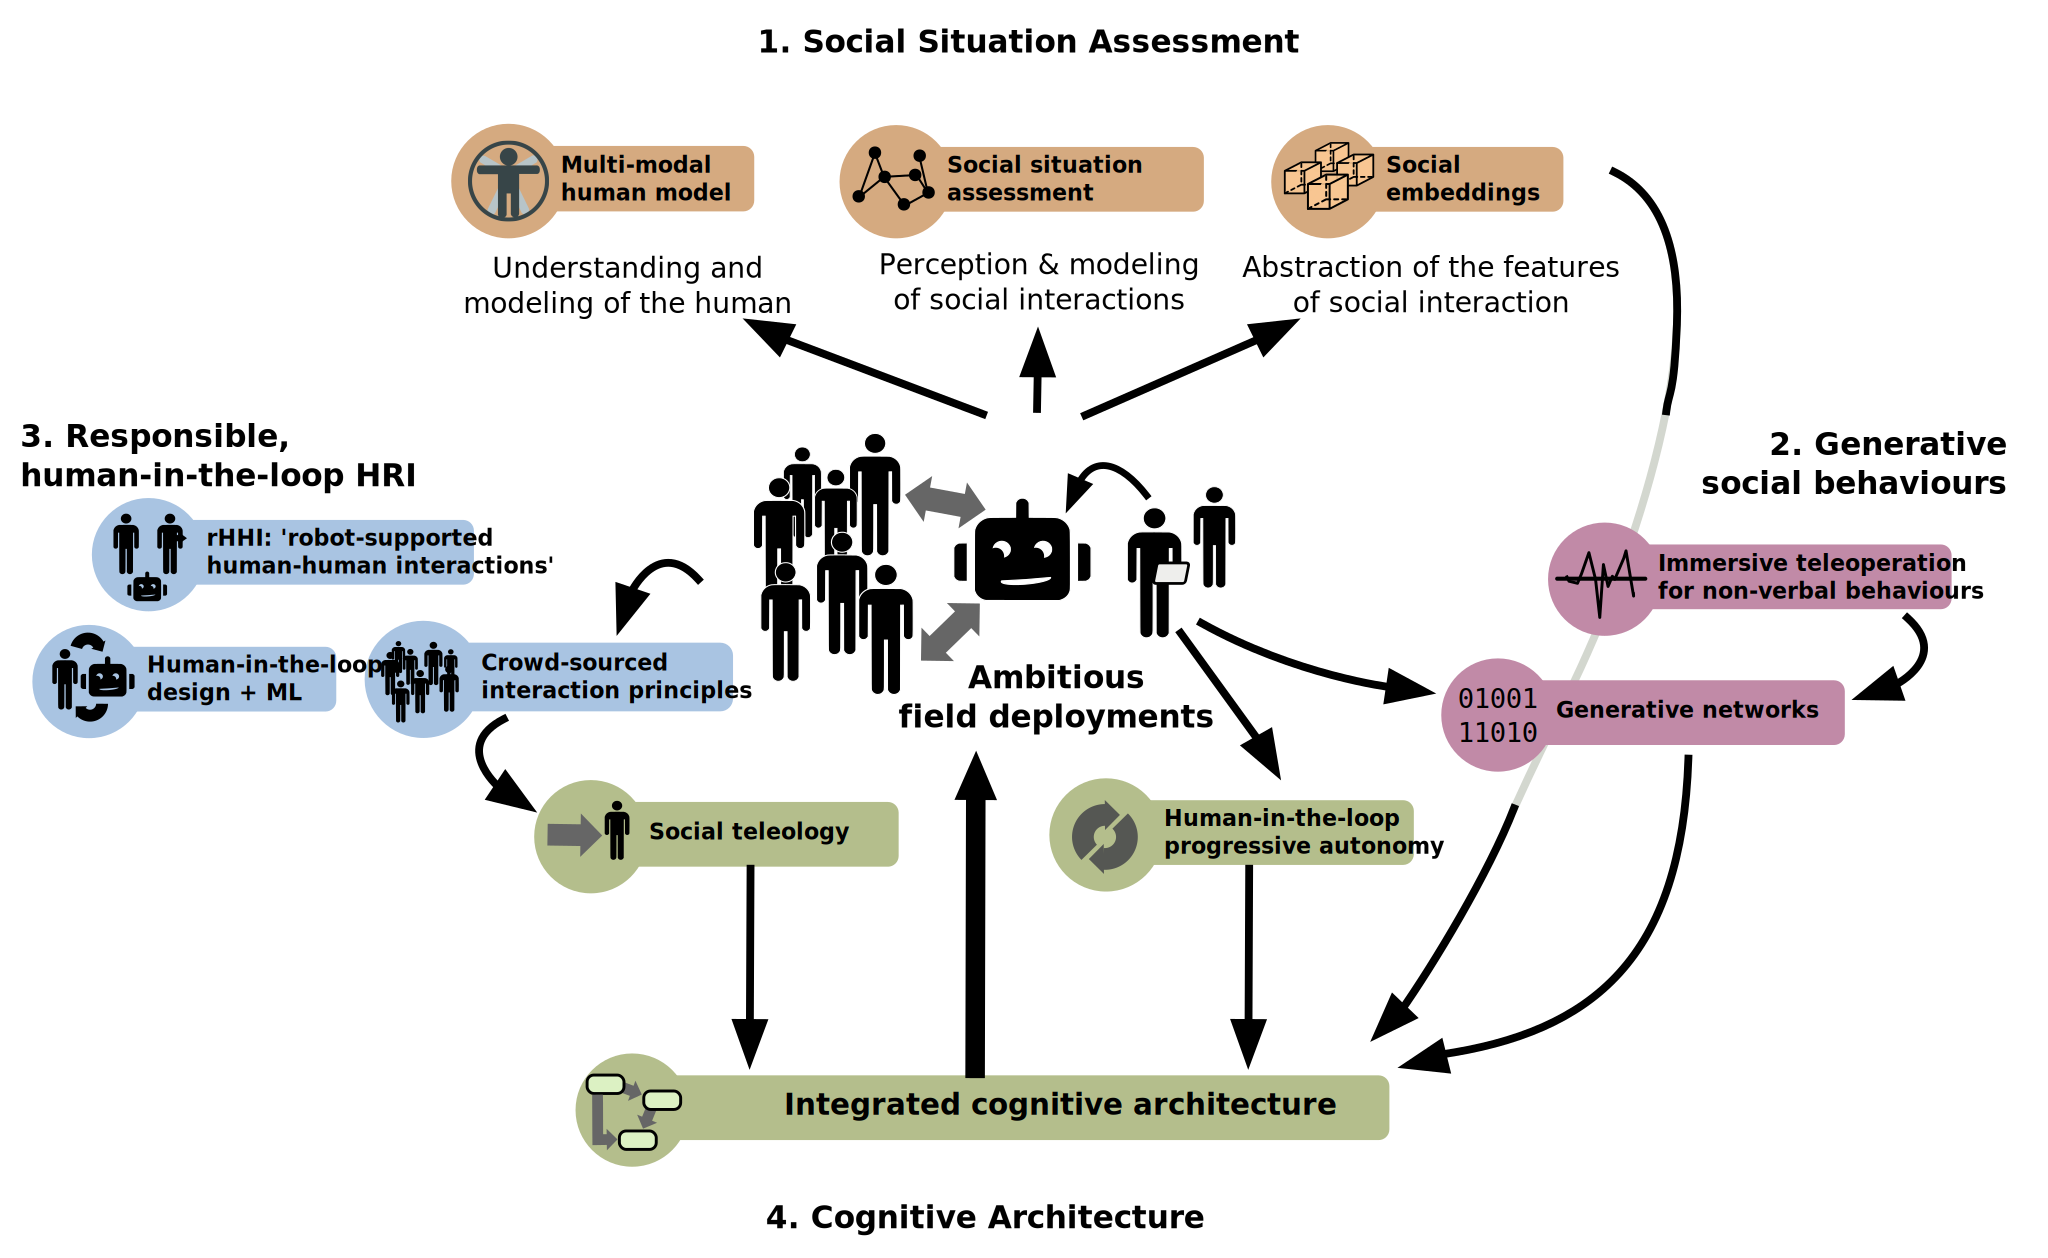
\includegraphics[width=0.7\linewidth]{architectures/wps.pdf}
        %        \hspace{1em}
        %    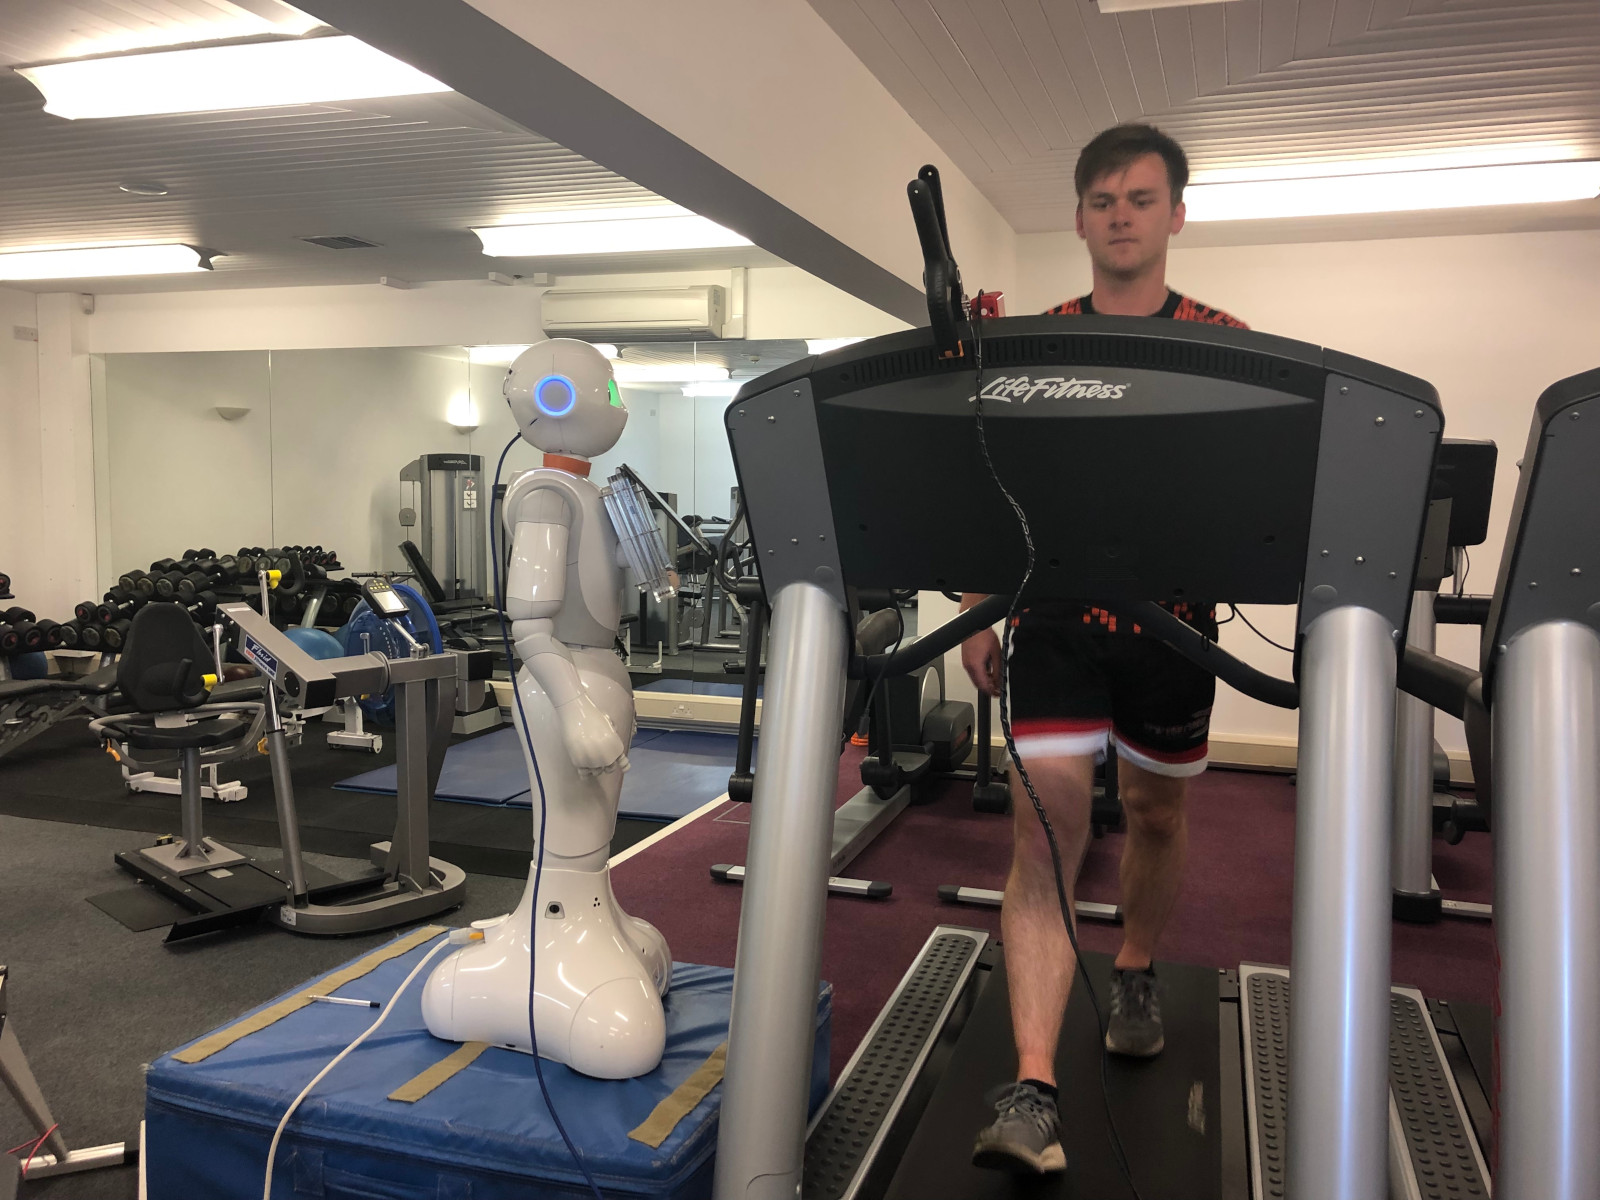
\includegraphics[trim=4cm 0 3cm 0,clip,width=0.25\linewidth]{couch25k/hri.jpg}
        %}
    \end{center}

    \begin{enumerate}
            \scriptsize
        \item beyond state-of-art \textbf{robust real-world social modelling}; \textbf{social embeddings}
        \item \textbf{public-in-the-loop} approach to design of \textbf{intrinsic social motivation}
        \item \textbf{generative social behaviours} for robots
        \item \textbf{cognitive architecture} for \textbf{long-term interaction}
    \end{enumerate}

\end{frame}


\begin{frame}{Idea: social embeddings}
    \begin{columns}
        \begin{column}{0.5\linewidth}
    \begin{center}
        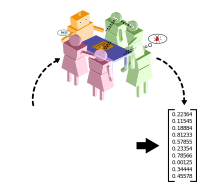
\includegraphics[width=\linewidth]{social-interactions/social-embeddings}
    \end{center}

        {\scriptsize
        \textbf{social embeddings}: learning a compact, sub-symbolic representation of social interactions
        }
        \end{column}
        \begin{column}{0.5\linewidth}
            \begin{itemize}
                \item real-world social interactions are highly dynamic, noisy,
                    multi-modal
                \item hard for the robot to model and reason about
                \item $\rightarrow$ \textbf{learn an embedding}: Attention nets, Deep
                    graph nets
                \item can be used by the robot to \textbf{recognise social situation} and
                    \textbf{generate congruent social behaviours}
            \end{itemize}
        \end{column}
    \end{columns}
\end{frame}

\begin{frame}{Idea: generative non-repetitive social behaviours}

    \centering
    \begin{columns}
        \begin{column}{0.6\linewidth}
            \centering
            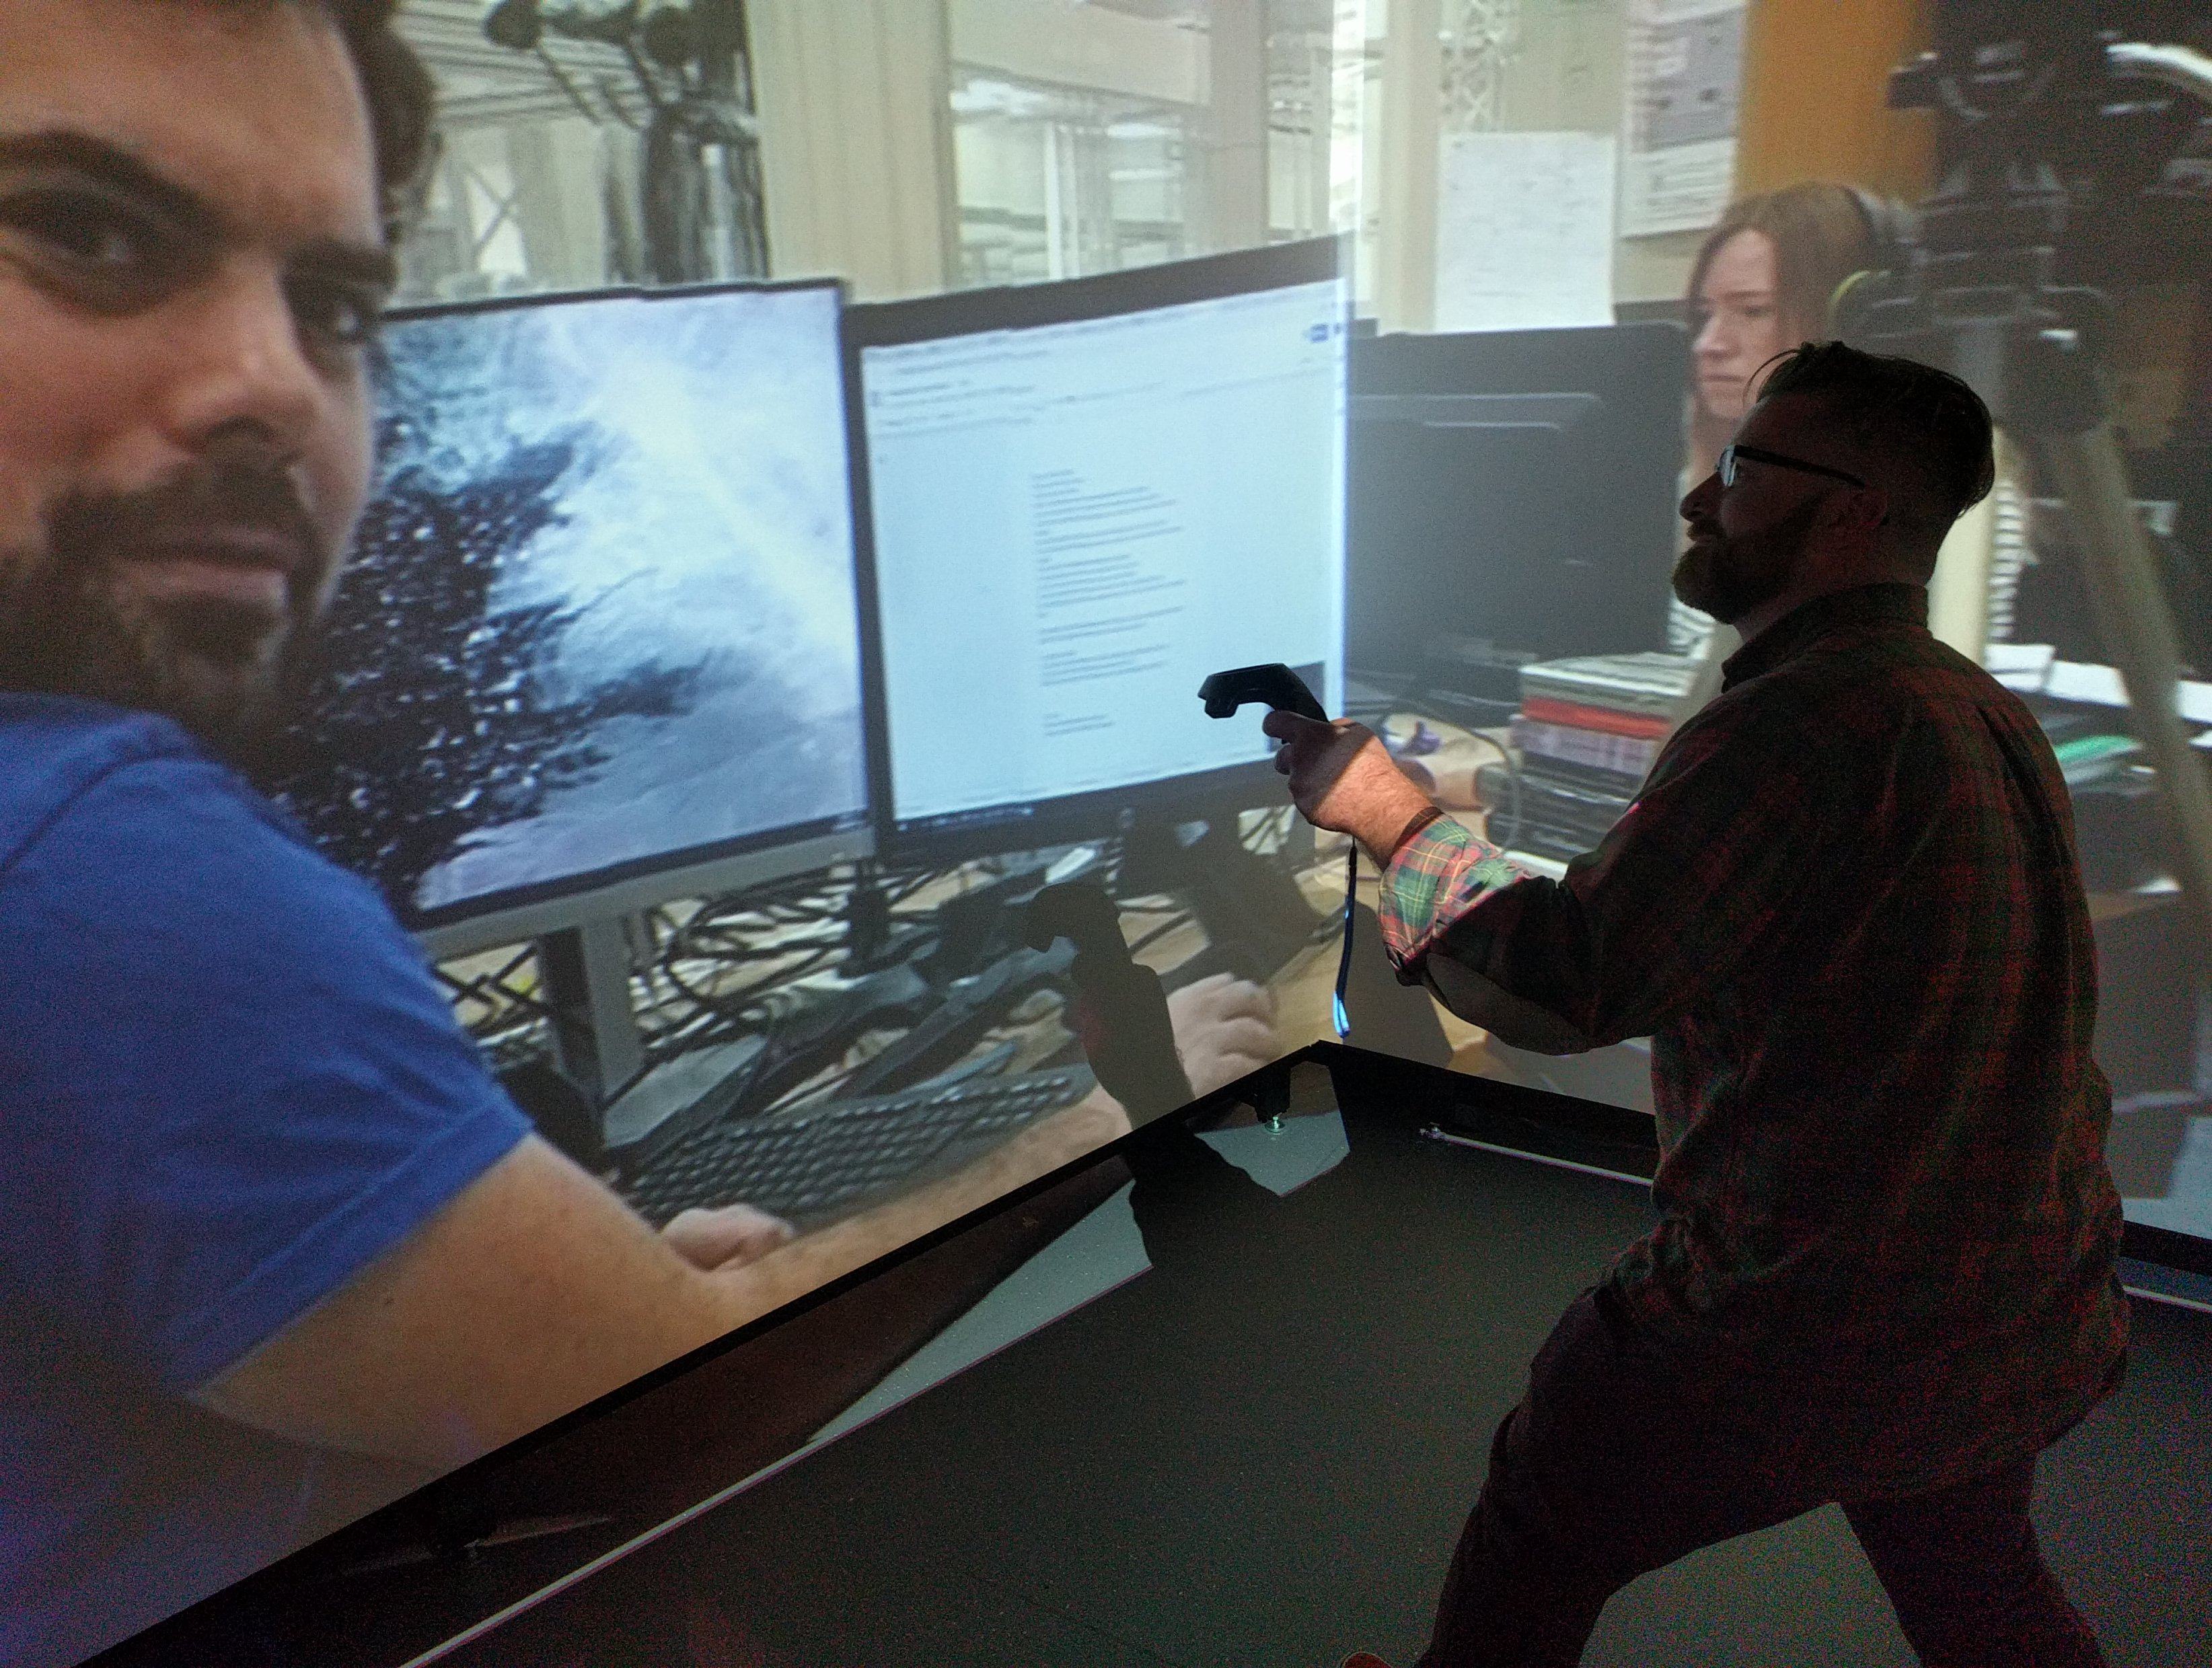
\includegraphics[width=.7\linewidth]{generative-behaviours/immersive-teleoperation}
        \end{column}
        \begin{column}{0.4\linewidth}
            \centering
            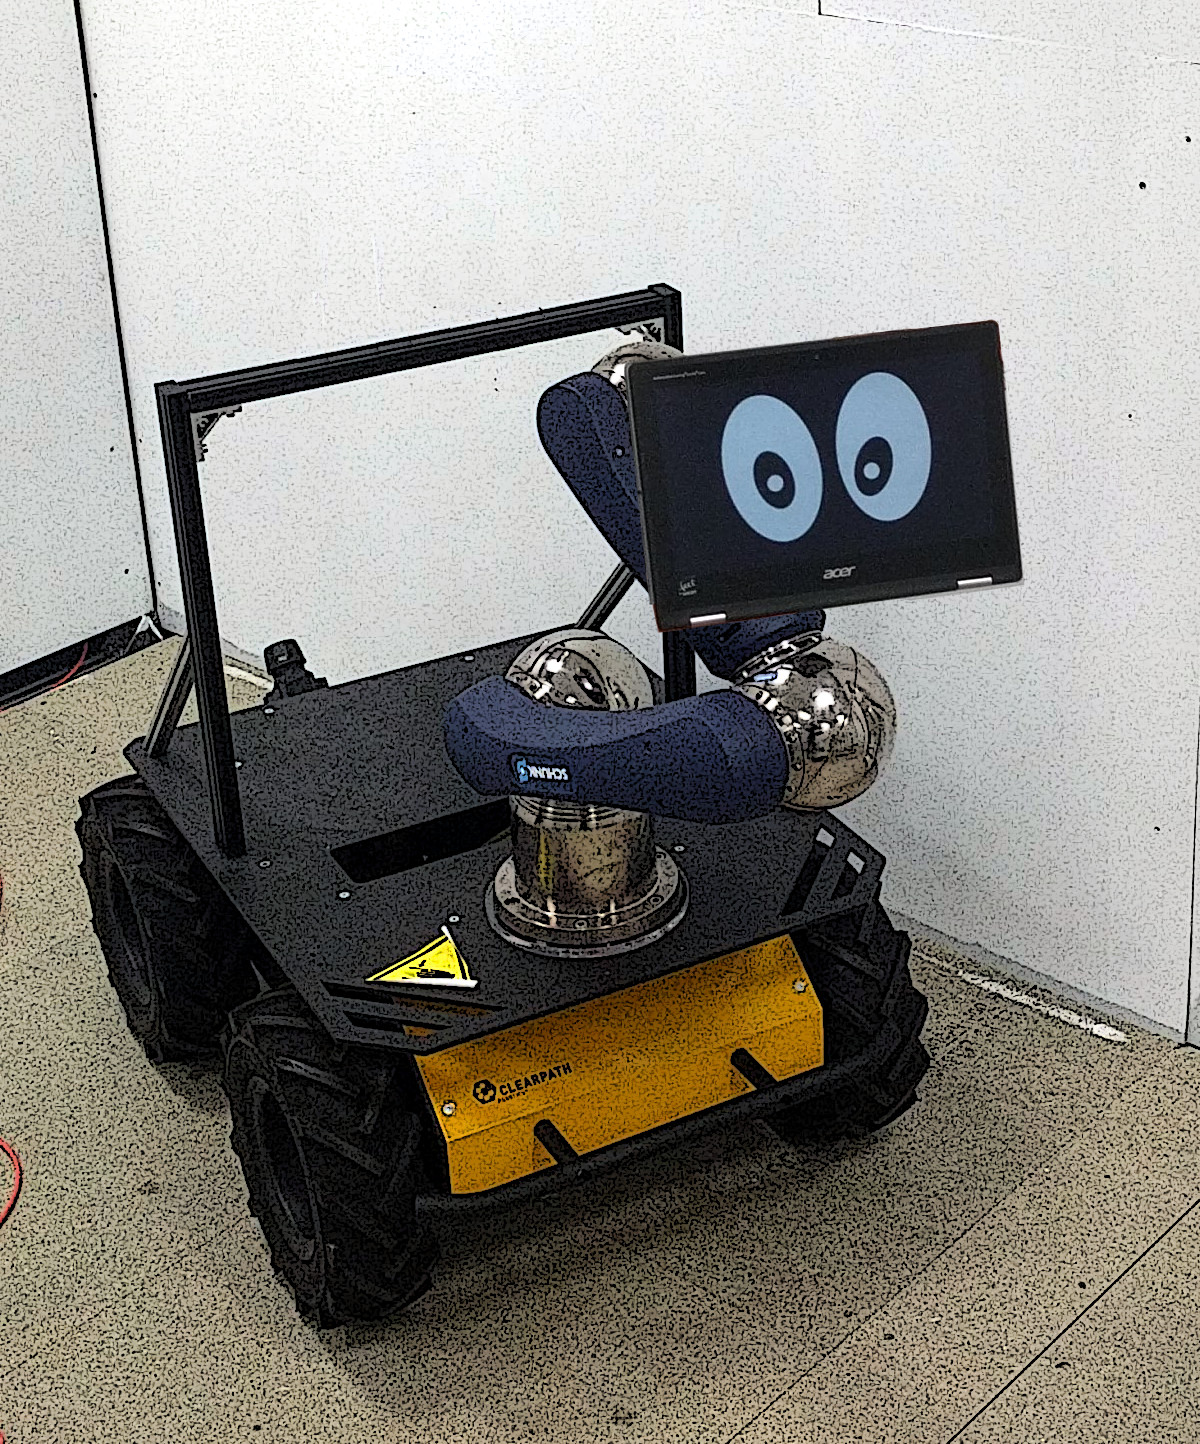
\includegraphics[height=4cm]{generative-behaviours/husky}
        \end{column}
    \end{columns}

    \vspace{1em}

            \scriptsize
            \begin{itemize}
                \item Cracking the `\textbf{non-repetitive, socially congruent}' behaviour
                    generation problem
                \item Extend \textbf{Generative Adversarial Networks} \emph{à la} AppGAN to complex
                    behaviours (re-use \emph{social embeddings})
                \item \textbf{Immersive technologies} to build datasets
                \item \textbf{Transdiscplinary approach}, incl. arts: choreographer, sound
                    expert
            \end{itemize}
\end{frame}

{
    \paper{Yang et al. \textbf{AppGAN: Generative Adversarial Networks for
    Generating Robot Approach Behaviours [...]} RoMan 2019}

\begin{frame}{Generative Adversarial Nets for behaviour generation}

    Some of the most exciting recent work in using ML for robot behaviour
    generation involve \textbf{Generative Adversarial Networks} (GANs):

            \begin{center}
                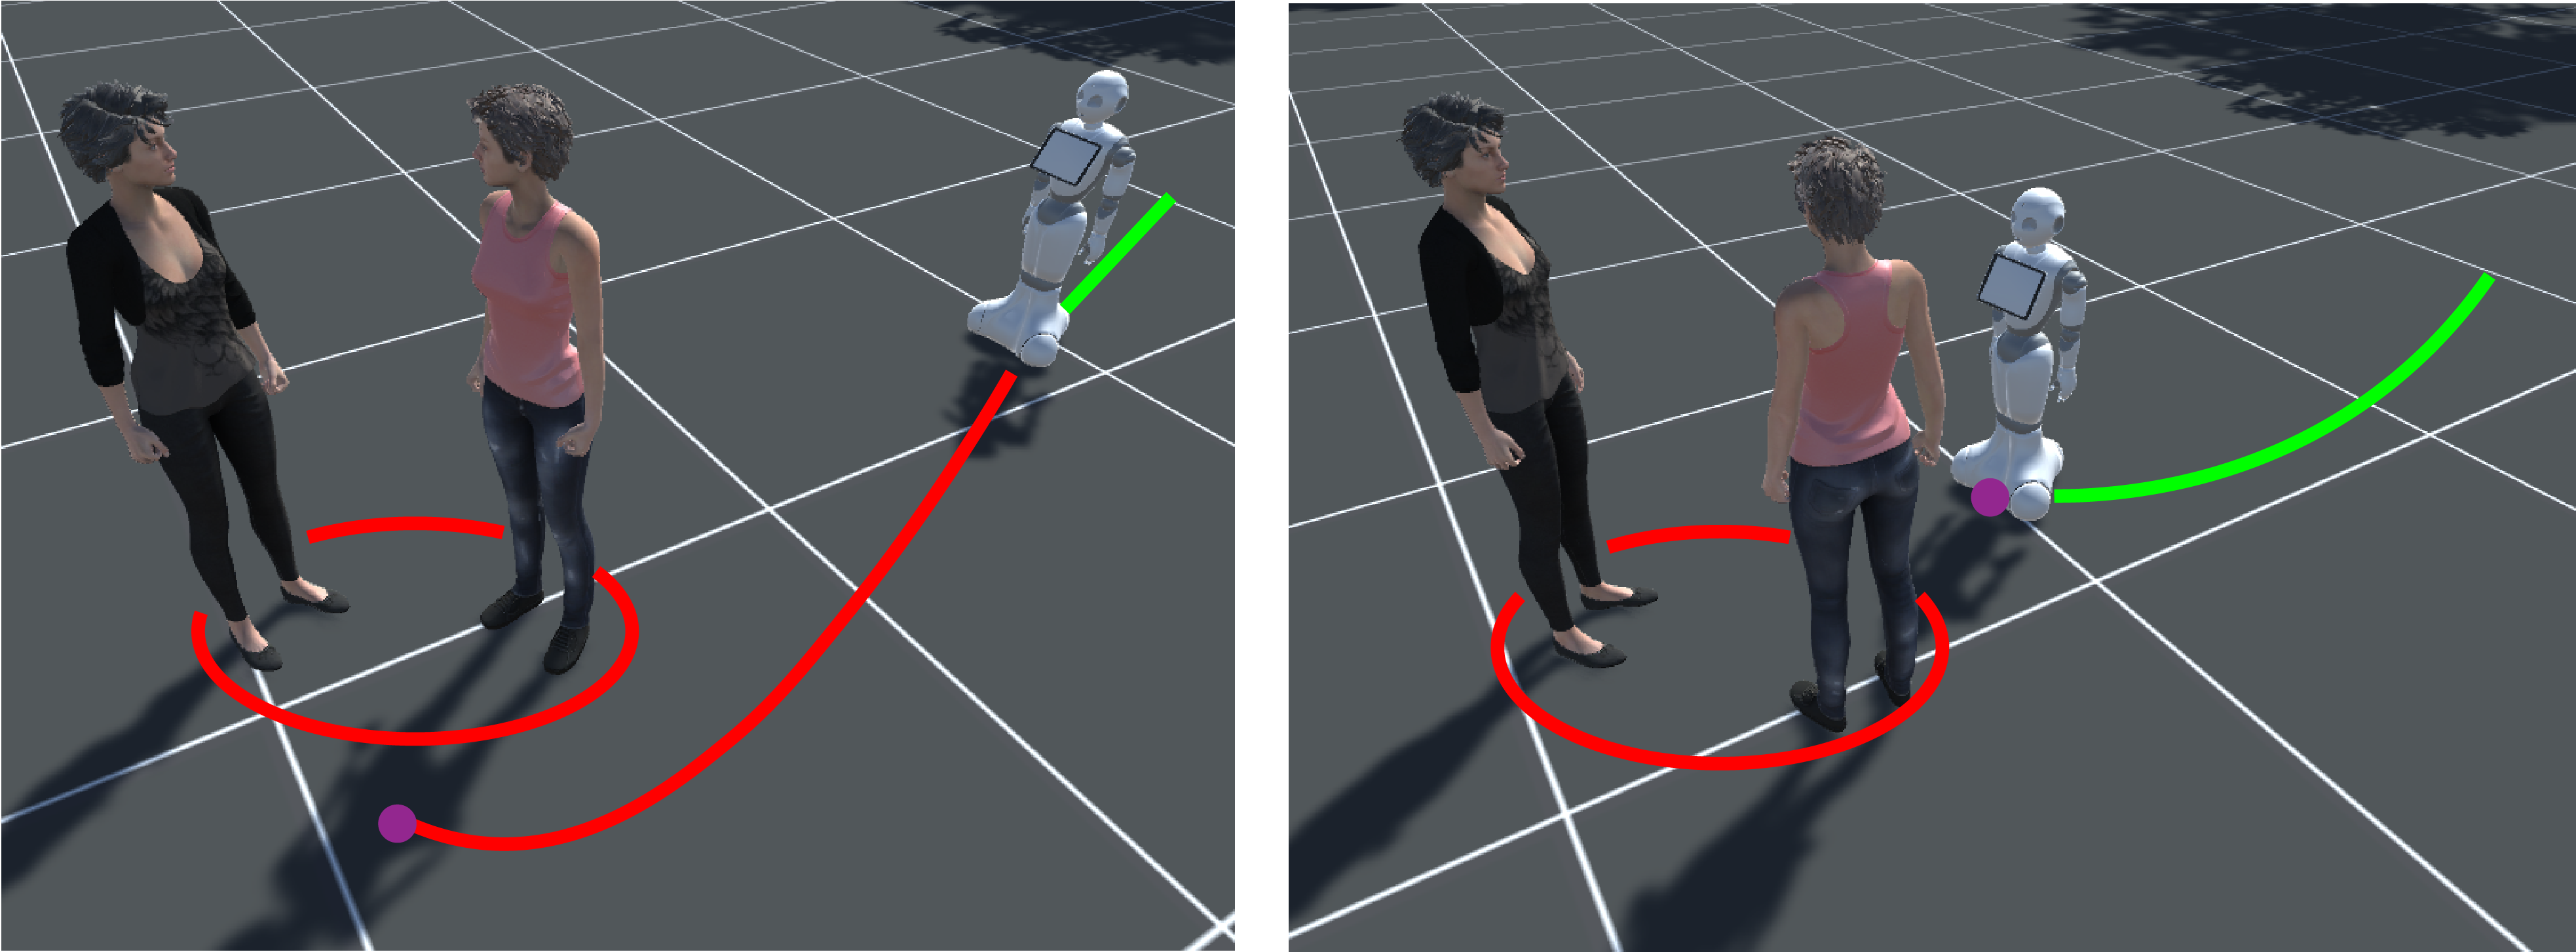
\includegraphics[width=0.6\linewidth]{figs/generation/fangkai-yang-appgan-traj.png}

                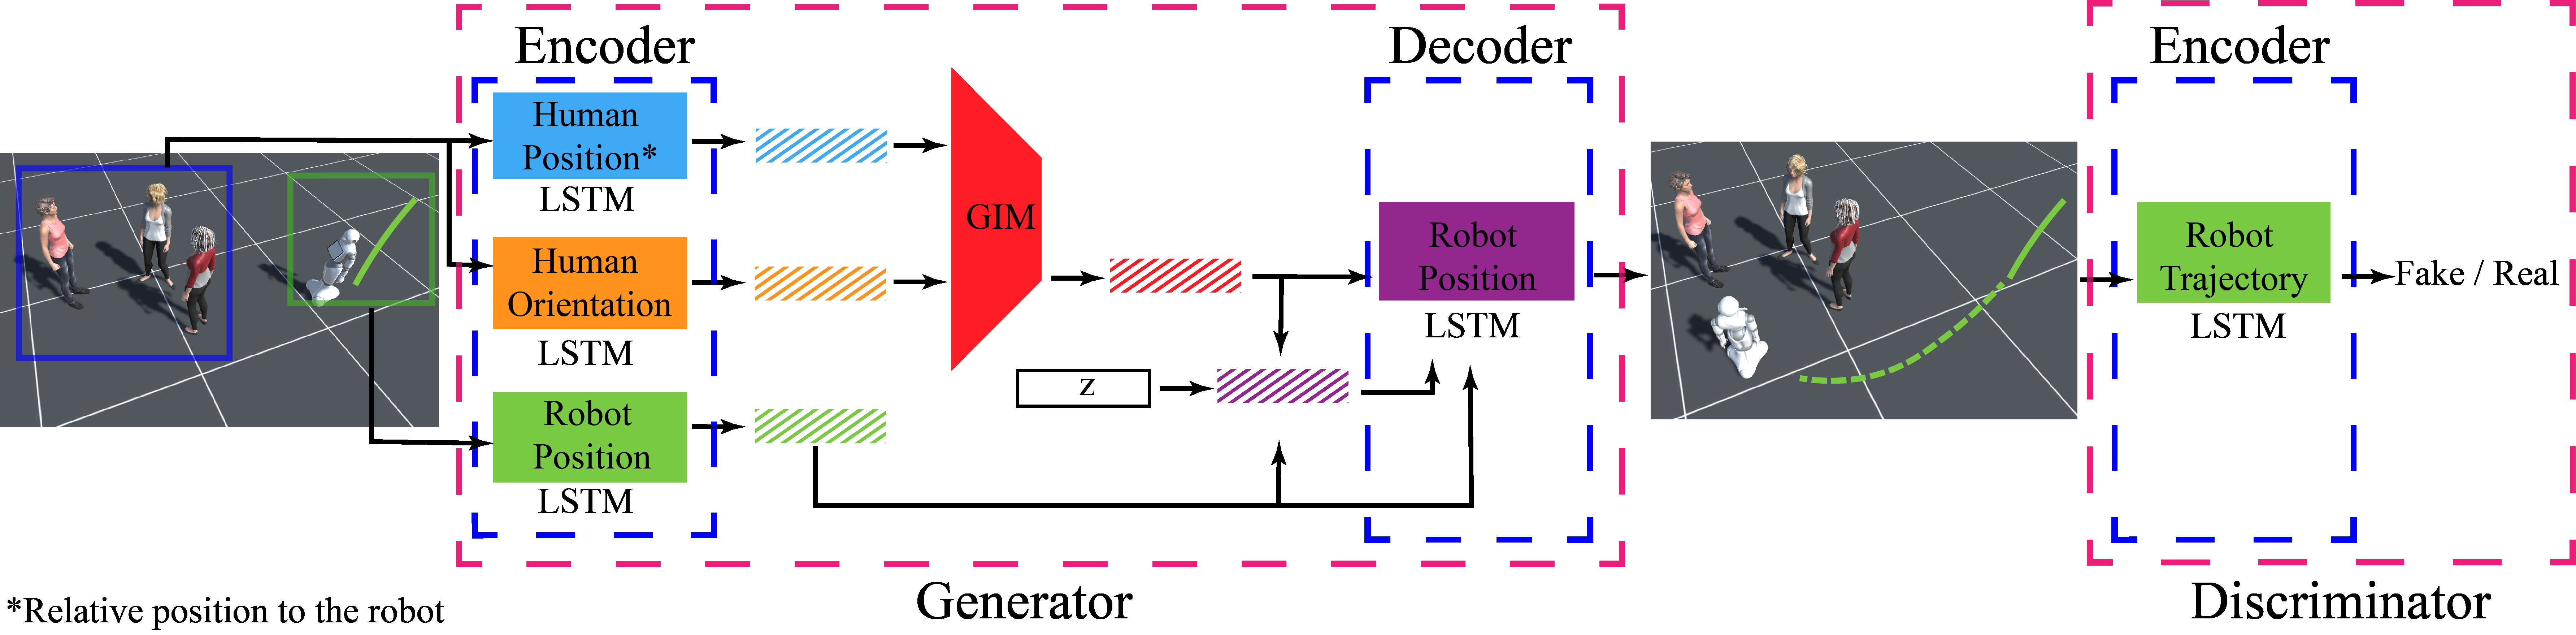
\includegraphics[width=0.8\linewidth]{figs/generation/fangkai-yang-appgan.png}
            \end{center}
\end{frame}
}

\begin{frame}[plain]

    \begin{center}
        \Large
 Cognitive architecture?
    \end{center}

\end{frame}

\imageframe[color=white]{islands1}

%%%%%%%%%%%%%%%%%%%%%%%%%%%%%%%%%%%%%%%%%%%%%%%%%%%%%%%%

\imageframe[color=white]{islands2}

%%%%%%%%%%%%%%%%%%%%%%%%%%%%%%%%%%%%%%%%%%%%%%%%%%%%%%%%

\imageframe[color=white]{islands3}

%%%%%%%%%%%%%%%%%%%%%%%%%%%%%%%%%%%%%%%%%%%%%%%%%%%%%%%%

\imageframe[color=white]{islands4}


\begin{frame}{Idea: socio-teleological architecture}

    \emph{Teleological} $\rightarrow$ \textbf{goal-oriented} architecture

    \begin{center}
        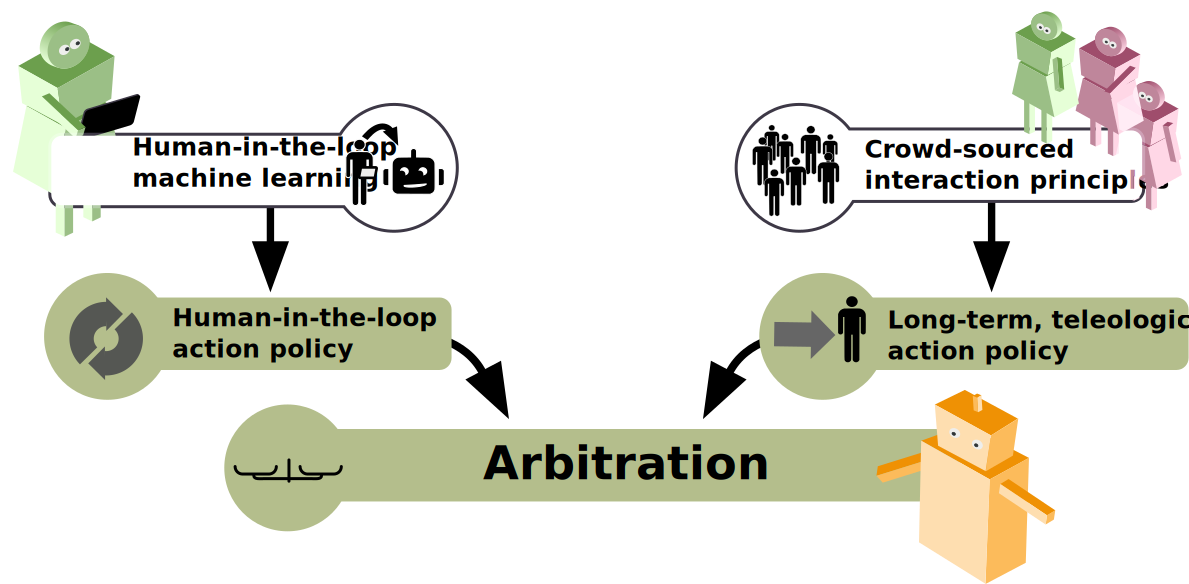
\includegraphics[width=0.8\linewidth]{architectures/arbitration}
    \end{center}

    \begin{itemize}
            \scriptsize
        \item \textbf{end-users and public to play a key role}:
        \item \textbf{crowd-sourced pro-social goals} (eg `show attention', `appear
            alive') drives long-term behaviours
        \item \textbf{short-term/domain-specific policies learned} via
            interactive reinforcement learning (IRL)
        \item \textbf{cognitive arbitration} between the two, based on
            \textbf{experience transfer}
    \end{itemize}
\end{frame}

\begin{frame}{Idea: robot-supported human-human interactions}
    \begin{center}
        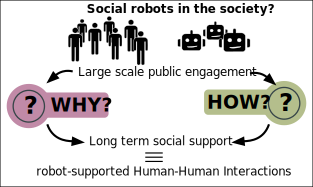
\includegraphics[width=0.5\linewidth]{figs/rHHI/rHHI}
    \end{center}

    Social robotics might need a paradigm shift from \emph{Human-Robot
    Interaction} to \textbf{robot-supported
    Human-Human Interaction}:
    \begin{itemize}
        \item not so much: how to robot can interact with human
        \item instead: why robots? what positive impact can robots uniquely
            deliver? (and \emph{then}: what technology is
            required)
    \end{itemize}
\end{frame}


\begin{frame}<1>[label=wps]{A HOLISTIC APPROCH TO SOCIAL ROBOTICS}
    \begin{center}
    \only<1>{
        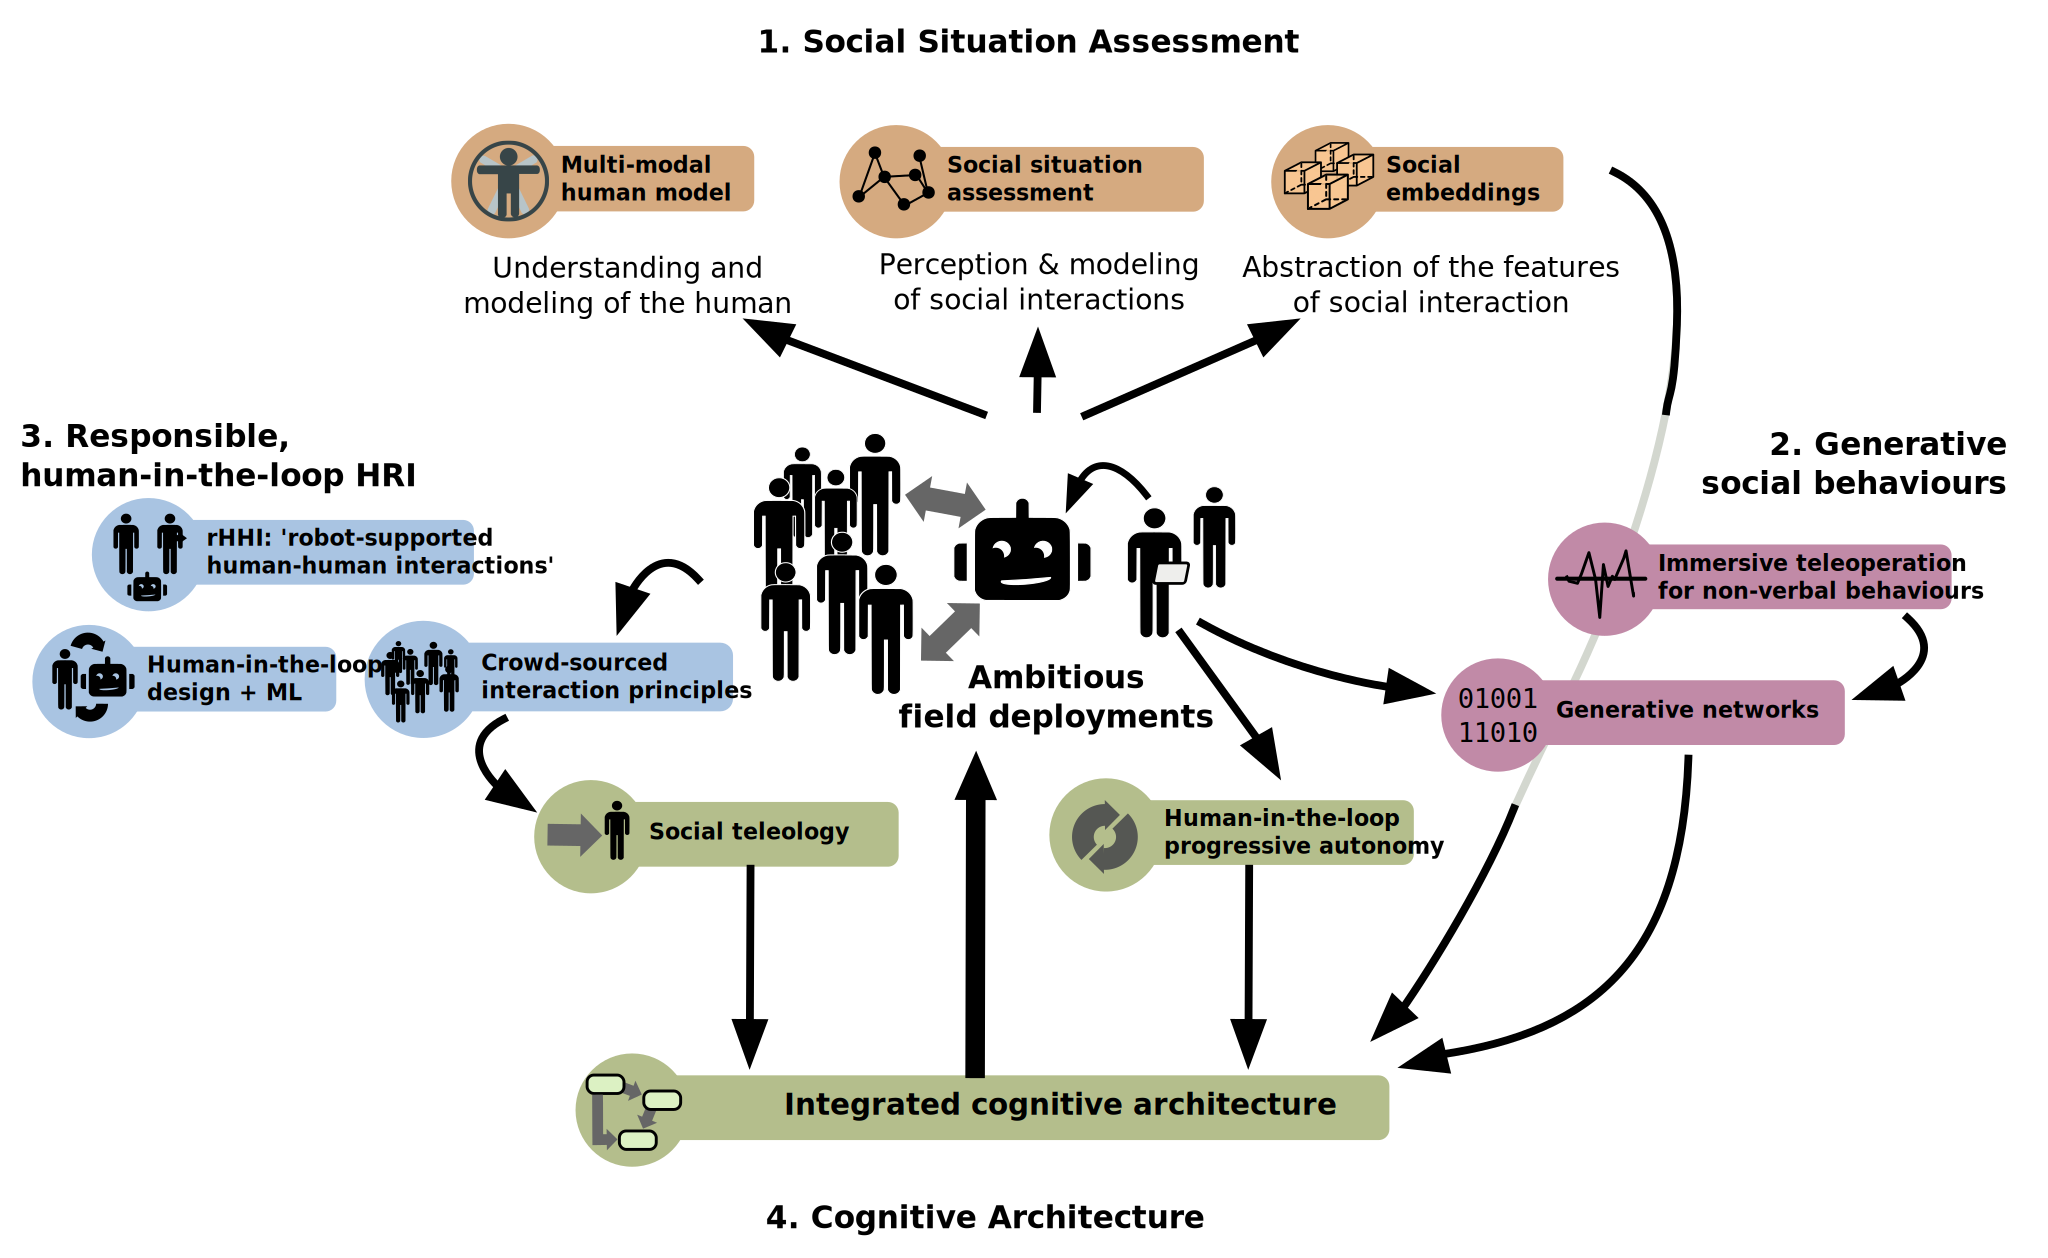
\includegraphics[width=\linewidth]{architectures/wps}
    }
    \only<2>{
        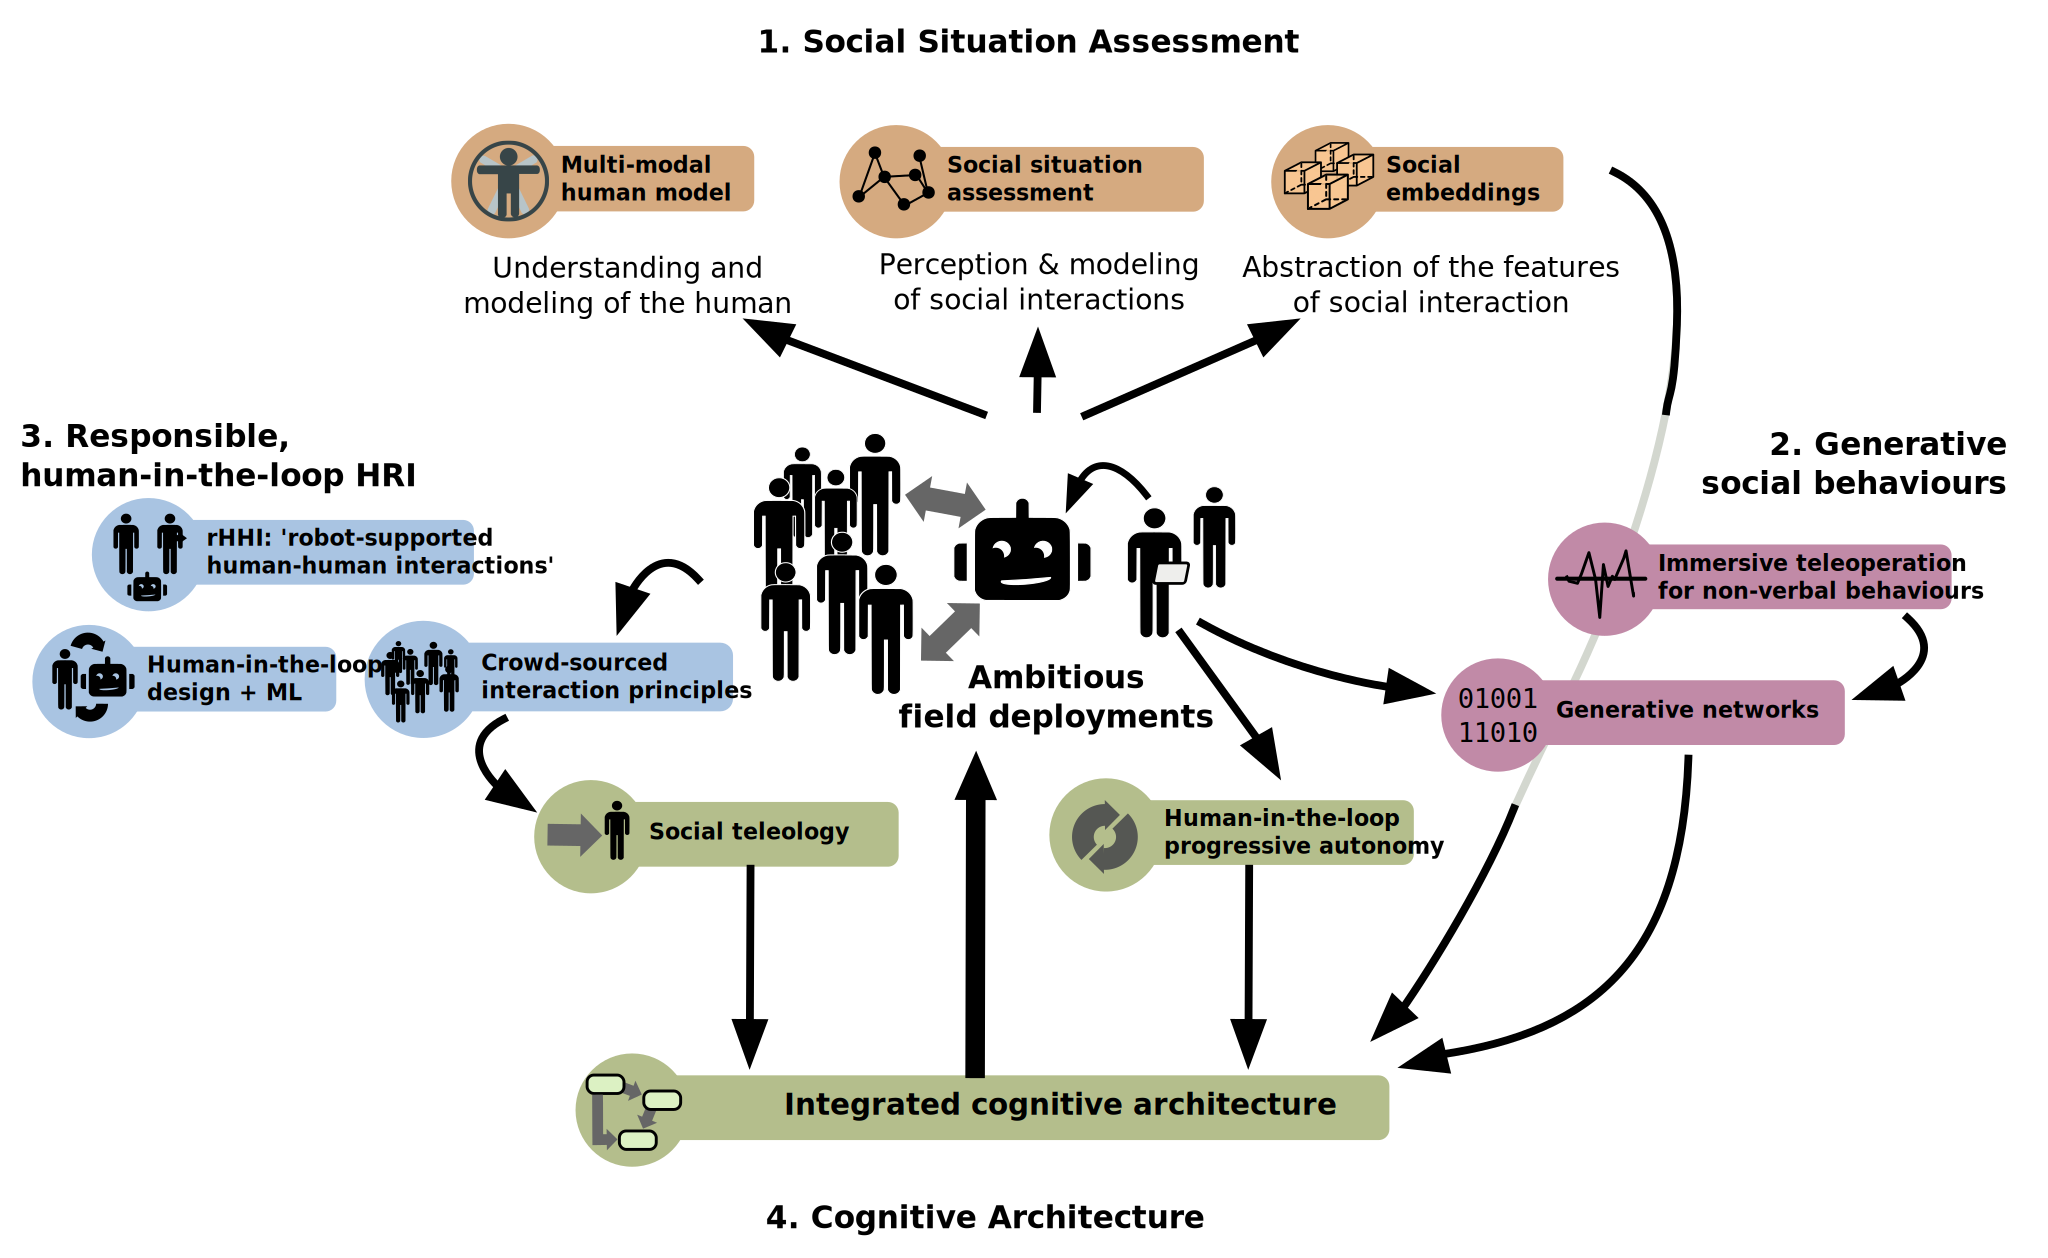
\includegraphics[trim=8cm 20cm 8cm 0,clip,width=\linewidth]{architectures/wps}
    }
    \only<3>{
        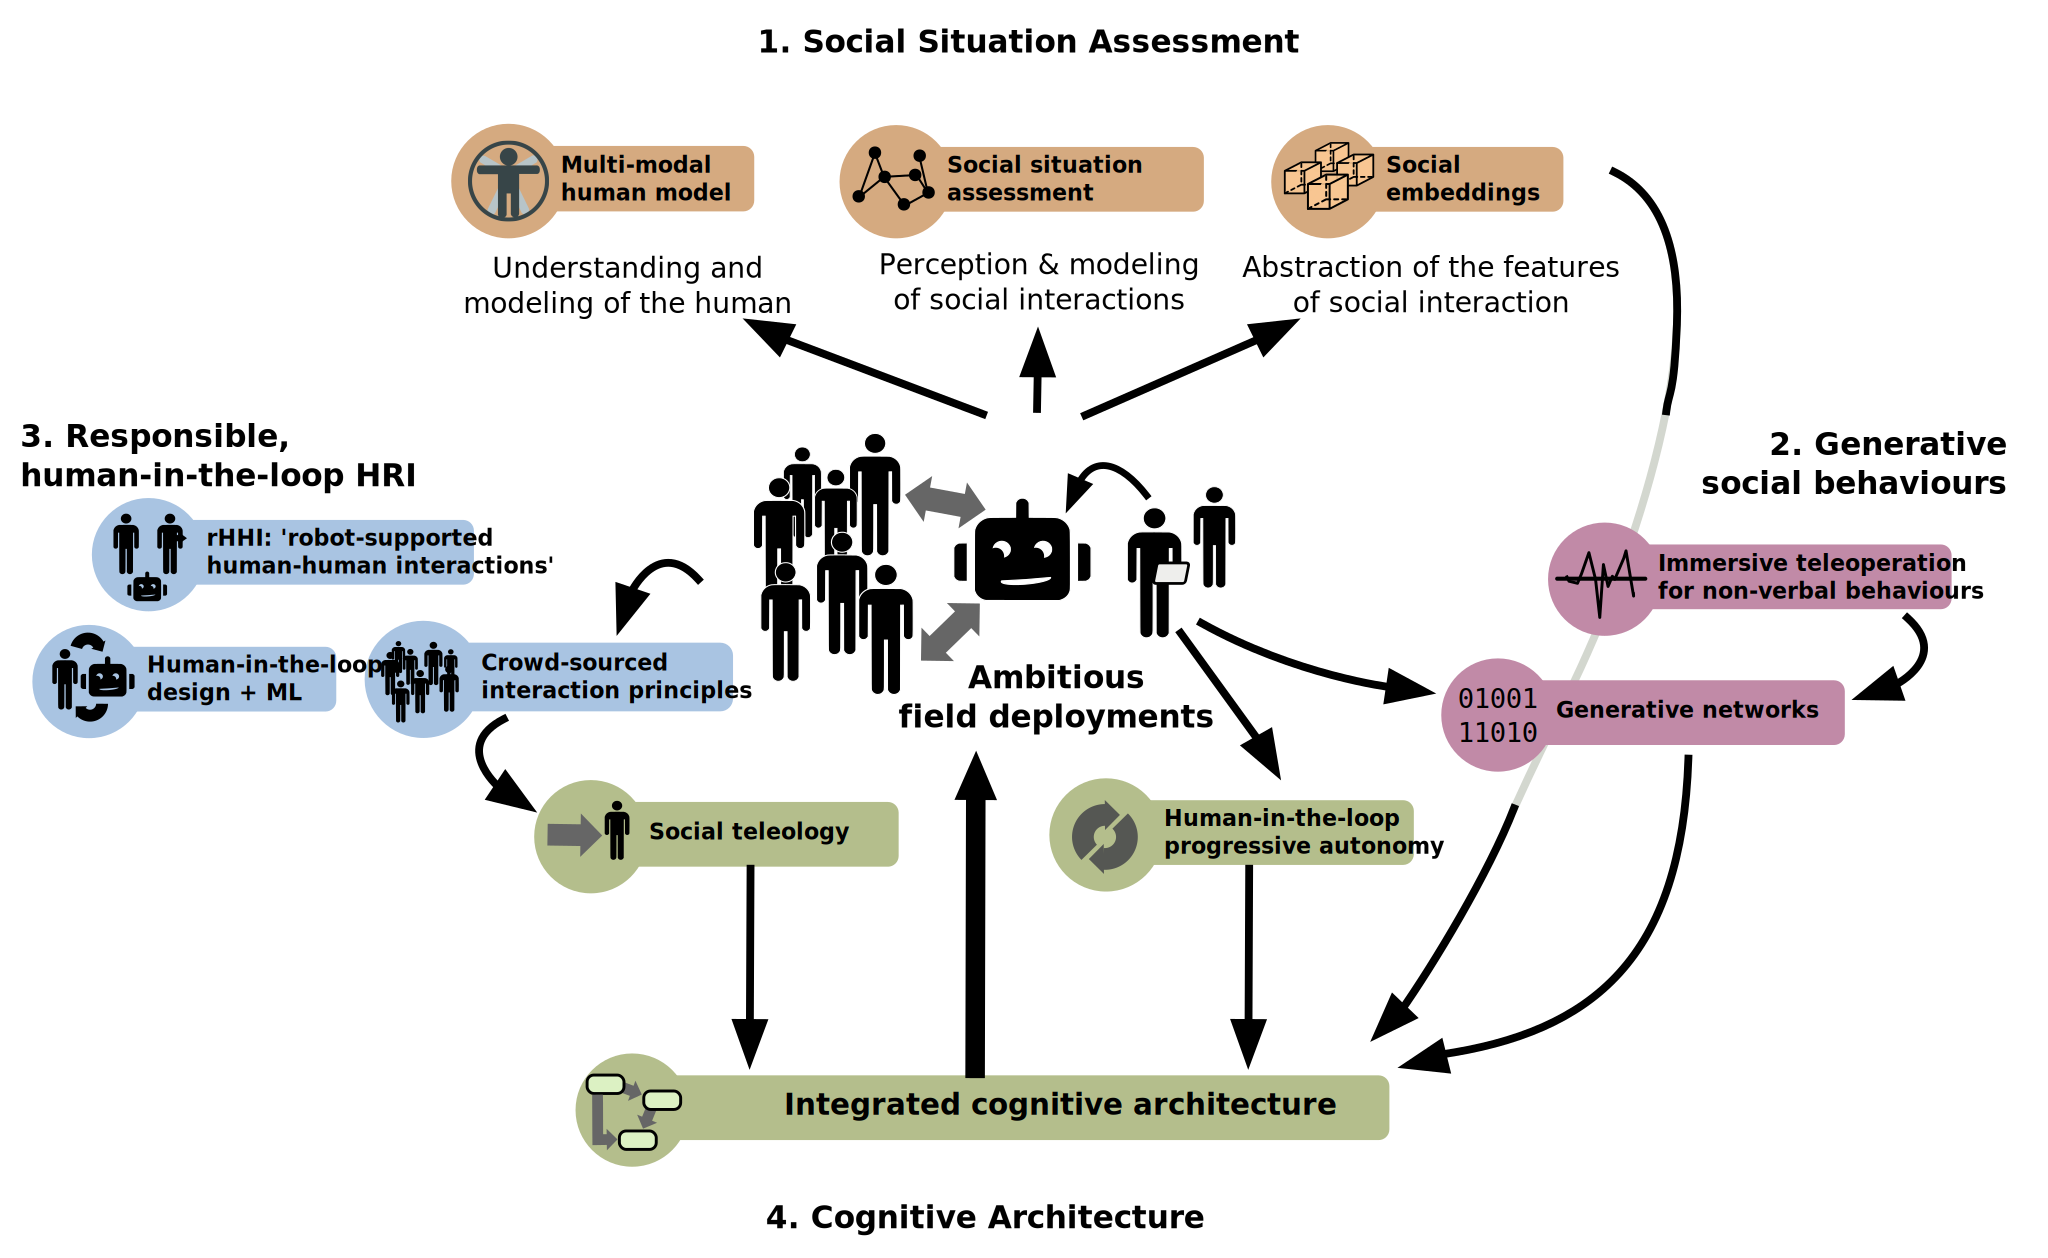
\includegraphics[trim=30cm 8cm 0 8cm,clip,width=0.7\linewidth]{architectures/wps}
    }
    \only<4>{
        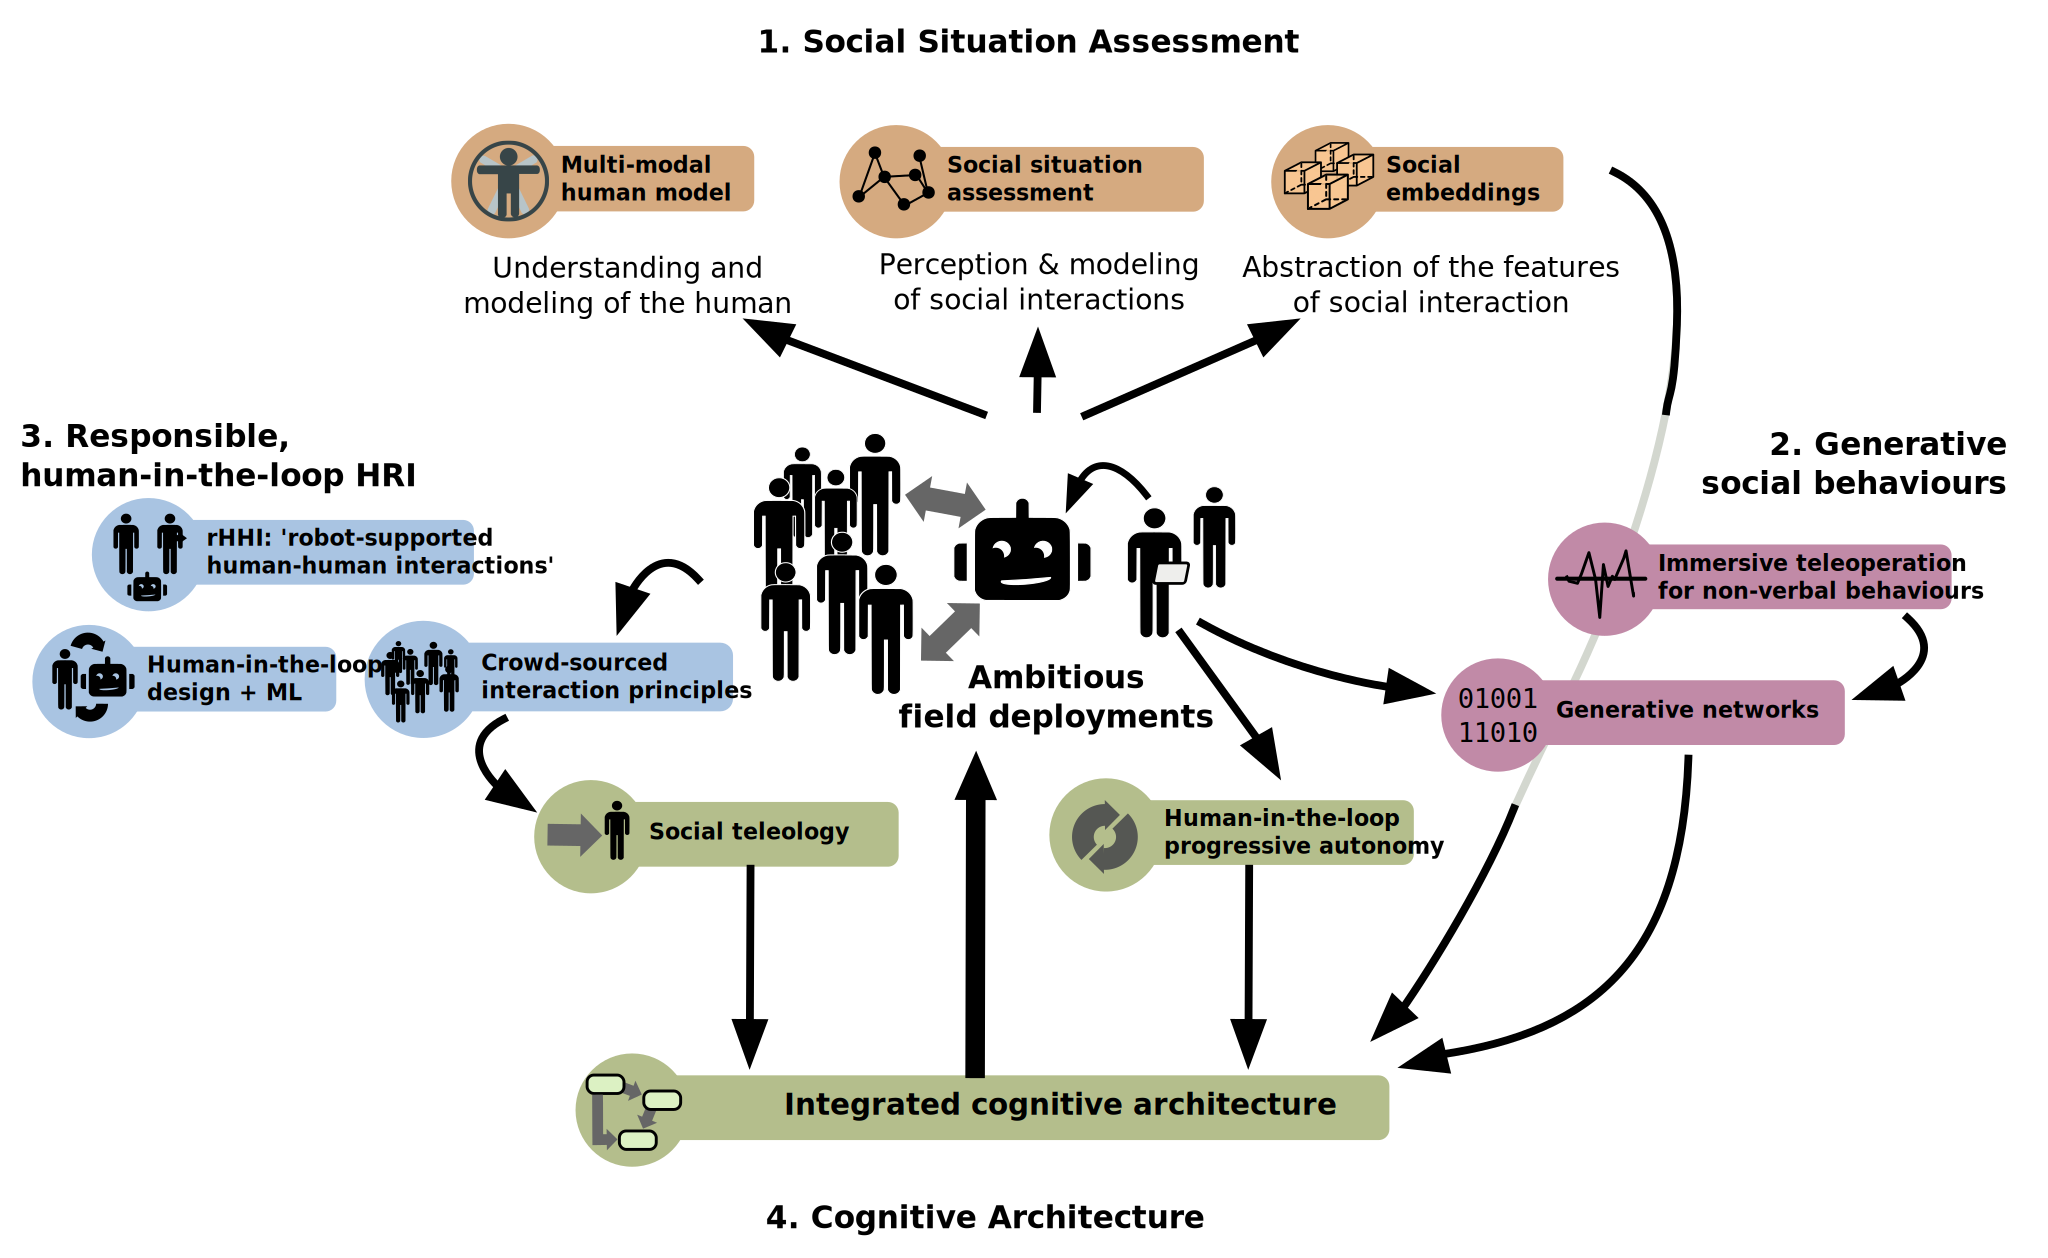
\includegraphics[trim=8cm 0 8cm 16cm,clip,width=\linewidth]{architectures/wps}
    }
    \only<5>{
        \includegraphics[trim=0 8cm 34cm 8cm,clip,width=0.7\linewidth]{architectures/wps}
    }
    \end{center}
\end{frame}

%%%%%%%%%%%%%%%%%%%%%%%%%%%%%%%%%%%%%%%%%%%%%%%%%%%%%%%%

{
    \fullbackground[color=black]{lastpage}
    \begin{frame}[plain]

        \begin{columns}
            \begin{column}{0.6\linewidth}
            \end{column}
            \begin{column}{0.4\linewidth}

                \setbeamercolor{hriSec1Demo}{fg=white!70!black}
                \vspace{6em}
                \begin{beamercolorbox}[wd=\linewidth,ht=6ex,dp=0.7ex]{hriSec1Demo}
                    \textbf{Thank you!}
                \end{beamercolorbox}
                \vspace{12em}
                {\scriptsize
                \textcolor{white!60!black}{(\emph{\textsc{roboscopie} 2012)}}
                }
            \end{column}
        \end{columns}
    \end{frame}
}

\end{document}
